\documentclass[a4paper,12pt]{report}
\usepackage[brazil]{babel} %Idioma
\usepackage[utf8]{inputenc}
\usepackage{amsmath,amsfonts,amsthm}
\usepackage[dvips]{graphicx}
\usepackage{rotating} % for sideways tables/figures
\usepackage[normalem]{ulem}
\usepackage{times} % modifica o estilo da página dos capítulos
\usepackage{boxedminipage} 
%\usepackage{amsthm}
\usepackage{graphicx}
\usepackage{wrapfig}
\usepackage{calrsfs}
\usepackage{multirow}
\usepackage{titlesec}
\usepackage{hyperref} % link interno e externo
\usepackage[width=7.00cm, height=3.00cm]{geometry}
\usepackage{color}
\usepackage{tikz}
\usepackage{float}
\usepackage{fancyheadings}
\usepackage{subfigure}
\usepackage{indentfirst}[1.25]
\usepackage{url}
\usepackage{setspace}
\usepackage{pdfpages}
 \usepackage{lipsum}
\setcounter{tocdepth}{6}
\setcounter{secnumdepth}{6}
\setlength{\textheight}{50pc}
\setlength{\textwidth}{38pc}
\setlength{\oddsidemargin}{0.5cm}
\setlength{\topmargin}{-0cm}

% Definição de alguns símbolos usados com frequência
\newcommand{\ini}{\noindent}
\newcommand{\inic}{\hspace{5.5mm}}
%
\newcommand{\bff}[1]{\boldsymbol{#1}}
\newcommand{\betab}{\bff{\beta}}
\newcommand{\mub}{\bff{\mu}}
\newcommand{\Sigmab}{\bff{\Sigma}}
\newcommand{\xb}{\bff{x}}
\newcommand{\Imb}{\bff{\Im}}
\newcommand{\etab}{\bff{\eta}}
\newcommand{\gammab}{\bff{\gamma}}
\newcommand{\Xb}{\bff{X}}
\newcommand{\Yb}{\bff{Y}}
\newcommand{\db}{\bff{d}}
\newcommand{\bb}{\bff{b}}
\newcommand{\cb}{\bff{c}}
\newcommand{\yb}{\bff{y}}
\newcommand{\Ob}{\bff{O}}
\newcommand{\varepsilonb}{\bff{\varepsilon}}
\newcommand{\alphab}{\bff{\alpha}}
\newcommand{\thetab}{\bff{\theta}}
\newcommand{\zetab}{\bff{\zeta}}
\newcommand{\deltab}{\bff{\delta}}
\newcommand{\Psib}{\bff{\Psi}}
\newcommand{\ab}{\bff{a}}
\newcommand{\taub}{\bff{\tau}}
\usepackage{makeidx}
\newtheorem{defin}{Definição}[section]
\newtheorem{teo}{Teorema}
\newtheorem{prop}{Proposição}[section]
\newtheorem{lema}{Lema}
\newtheorem{corolario}{Corolário}
\newcommand{\exemplo}{\textbf{Exemplo. }}
\newcommand{\exemploreso}{\textbf{Exemplo Resolvido. }}
\newcommand{\exercicio}{\textbf{Exercício}}
\usepackage{graphicx}
\renewcommand{\qedsymbol}{\rule{0.7em}{0.7em}}

\pagestyle{headings}
\pagenumbering{arabic}
\setcounter{page}{2}
\baselineskip=20pt %aumenta o espaçamento entre as linhas do texto
\begin{document}
%--------------- FOLHA DE ROSTO --------------- %
\thispagestyle{empty} \vspace{1cm}
%\vspace{0.5cm}
\begin{figure}[H]
	\centering
\includegraphics[scale=.25]{figuras/brasao_uemasul}
\end{figure}
\begin{center}
UNIVERSIDADE DA REGIÃO TOCANTINA DO MARANHÃO - UEMASUL \\
CAMPUS AÇAILÂNDIA - CCHSTL \\
\end{center}

\vspace{2.0cm}

\begin{center}
Andrey Brito Nascimento
\end{center}

\vspace{4.5cm}

\begin{center}
	\textbf{MATEMÁTICA BÁSICA PARA ENSINO SUPERIOR}
\end{center}

\vspace{7.5cm}

\centerline{\normalsize {\textbf{Açailândia/MA}}}%\vspace{1cm}
\centerline{\normalsize {\bf 2021}}
\tableofcontents
\setcounter{chapter}{0} %Instruções
% 1 - o pré ambulo esta arrumado para um formato padrão;
% 2 - Não mexer no arquivo main.

\chapter{Matemática Discreta}

\section{Notações}
 Para representar somas finitas ou infinitas fazemos uso do símbolo
 \begin{equation}
     \sum_{i=1}^{n} x_i = x_1 + x_2 + x_3 + \cdots + x_{n-1} + x_{n}.
 \end{equation}
\begin{example}

\begin{enumerate}
    \item [(i)] $\displaystyle \sum_{i=1}^{5} x_i = x_1 + x_2 + x_3 + x_{4} + x_{5}$;
    \item [(ii)] $\displaystyle \sum_{i=1}^{5} x_i = x_1 + x_2 + x_3 + x_{4} + \cdots + x_{10}$;
    \item [(iii)] $\displaystyle \sum_{i=1}^{300} x_i = x_1 + x_2 + x_3 + \cdots+ x_{299} + x_{300}$.
\end{enumerate}

\end{example}
\quad Em algum momento podemos nos deparar com:
\begin{equation}
\label{serie}
     \sum_{i=1}^{\infty} x_i = x_1 + x_2 + x_3 + \cdots,
 \end{equation}
a expressão (\ref{serie}) é chamada de série de números reais. 
\subsection{Propriedades}
Sejam os números reais $x_i$ e $y_i$ com $i = 1,2,3,\cdots,n$ escalares $\alpha$ e $\beta$, temos 
\begin{enumerate}
    \item [(i)] $\displaystyle \sum_{i=1}^{n} (\beta x_i\pm \alpha y_i) = \displaystyle \beta \sum_{i=1}^{n} x_i \pm \displaystyle \alpha \sum_{i=1}^{n} y_i $;
    \item[(ii)] $\displaystyle \sum^n_{i = m} \sum^\ell_{j = k} x_iy_j = \sum^n_{i = m} x_i\sum^\ell_{j = k} y_j$;
    \item[(iii)] $\displaystyle \left|\sum^n_{i = 1} x_i \right| \leq  \sum^n_{i = 1} |x_i|$, em particular para $x_1$ e $x_2$ temos $|x_1 + x_2| \leq |x_1| + |x_2|$ a conhecida desigualdade triangular.
    \item[(iv)] Dada as funções diferenciáveis $f_i: \mathbb{R} \rightarrow \mathbb{R}$ temos $\displaystyle \sum^n_{i = 1}  \frac{\partial f_i(x)}{\partial x_i} = \frac{\partial \displaystyle }{\partial x_i}\sum^n_{i = 1}f_i(x) $  
     
\end{enumerate}

Será necessário representarmos o produto de $n$ números, da sequência $\{x_n\}_{n\in \mathbb{N}}$, que será feita pelo símbolo.

\begin{equation}
    \prod_{i=1}^{n} x_i = x_1x_2x_3\cdots x_n,
\end{equation}

\noindent o desenvolvimento deste simbolo se dá semelhante ao especificado nos exemplos de somatório. 

\subsection{Propriedades}
Considere novamente uma sequência de número reais $\{x_n\}_{n\in \mathbb{N}}$
\begin{enumerate}
    \item [(i)] $\displaystyle \prod_{i=1}^{n} (\beta x_iy_i) = \displaystyle \beta^n \prod_{i=1}^{n} x_i \displaystyle \prod_{i=1}^{n} y_i $;
    \item[(ii)] $\displaystyle \left(\prod^n_{i = 1}  x_i\right)^p = \displaystyle \prod^n_{i = 1}  x_i^p$;
    \item [(iii)] $\displaystyle \prod^n_{i = 1}  (x_i + y_i) \geq \displaystyle \prod^n_{i = 1}  x_i + \displaystyle \prod^n_{i = 1}  y_i$; 
    \item[(iv)] $\displaystyle\log \prod^n_{i = 1}  x_i =  \sum^n_{i = 1}\log x_i$ em particular para $n=2$ temos $\log x_1x_2 = \log x_1 + \log x_2$.
\end{enumerate}

\section{Indução Finita}
\inic Indução finita é uma poderosa técnica matemática de demonstração que é baseada nos axiomas de Peano, um matemático que buscou formalizar as ideia de números naturais que são os números usados para contagem $\mathbb{N} = \{1,2,3,4,\cdots\}$ ou $\mathbb{N} = \{0,1,2,3,4,\cdots \}$, é importante enfatizar que ainda não há um consenso (e acho que nunca haverá) se o zero é um número natural, todavia nestas notas de aula usaremos o zero quando conveniente. Enunciaremos agora os axiomas de Peano.

\subsection{Axiomas de Peano}
\inic Os números naturais são caracterizados pelos seguintes fatos:
\begin{enumerate}
    \item [(i)] Todo número natural tem um sucessor, que ainda é um número natural; números diferentes têm sucessores diferentes;
    \item[(ii)] Existe um único número natural 1 que não é sucessor de nenhum outro;
    \item[(iii)] Se um subconjunto dos naturais contem o número 1, e para qualquer outro elemento contem também o seu sucessor, então esse conjunto contém também todos os naturais.
\end{enumerate}
\inic Estes três axiomas formalizam a ideia matemática de número natural. Para melhor entendimento do axioma (iii), pense em uma fileira infinita de dominós, em que você está interessado em derrubar todos os dominós, para fazer isso você precisa derrubar o primeiro (contem o número 1) e depois garantir que para qualquer dominó no meio da fileira (n) você este irá derrubar o próximo (sucessor), e assim você garante que a fileira toda cairá. De fato mostraremos alguns clássicos exemplos de como utilizar esta técnica para demonstrações, e apresentaremos alguns passos para utiliza-la:

\begin{enumerate}
    \item [(a)] Mostre que a propriedade é válida para $n=1$ (base de indução);
    \item[(b)] Suponha que a propriedade é válida para $n$ (Hipótese de indução);
    \item[(c)] Mostre que a propriedade é válida para $n+1$ (sucessor de $n$) e conclua que vale para todo $n$.
\end{enumerate}
\inic Apresentaremos agora alguns exemplos de como aplicar esses passos.

\begin{example}
 Prove as identidades abaixo (o zero aqui não é natural):
    \begin{enumerate}
        \item [(a)] $1+2+3+\cdots+n = \frac{n(n+1)}{2}, \forall n \in \mathbb{N}$;
        \item [(b)] $1+3+5+\cdots+2n-1 = n^2, \forall n \in \mathbb{N}$
        \item [(c)] $1^2 + 2^2 + 3^2 +... + n^2 = \frac{n(n+1)(2n+1)}{6}, \forall n \in \mathbb{N}$;
        \item [(d)] $1^3 + 2^3 + 3^3 +... + n^3 = \frac{n^2(n+1)^2}{4}, \forall n \in \mathbb{N}$;
        \item [(e)] $4^n >n^4$, $\forall n \geq 5$;
        \item [(f)] $n! > n^3$, $\forall n \geq 6$.
    \end{enumerate}
\end{example}
\inic Provaremos aqui as letras (a) e (e), os demais exemplos ficam como exercícios para o leitor.

\begin{proof}
(a) Provaremos por indução, logo substituindo $n=1$ [Passo (a)] temos
$$1 = \frac{1(1+1)}{2},$$
logo a identidade é verdadeira para $n=1$.
Suponha então que seja verdade [Passo (b)] que
$$1+2+3+\cdots+n = \frac{n(n+1)}{2},$$
agora vamos provar que vale para $(n+1)$ [Passo (c)], assim somaremos o termo sucessor em ambos lados da igualdade, logo
$$1+2+3+\cdots+n + (n+1) = \frac{n(n+1)}{2} + (n+1)$$

$$1+2+3+\cdots+n + (n+1) = \frac{n^2+n + 2n+2}{2}$$
$$1+2+3+\cdots+n + (n+1) = \frac{n^2+3n+2}{2}$$
Podemos fatorar o polinômio $n^2+3n+2 = (n+1)(n+2)$ logo
$$1+2+3+\cdots+n + (n+1) = \frac{(n+1)(n+2)}{2}$$
$$1+2+3+\cdots+n + (n+1) = \frac{(n+1)[(n+1)+1]}{2}$$
\noindent o que prova a identidade.
\end{proof}

\begin{proof}
(e) Provaremos para $n=5$, de fato 
$$4^5 > 5^4 \Rightarrow 1024 > 625,$$
a base de indução foi provada. Agora suponha verdadeiro que 
$$4^n > n^4,$$
agora provaremos que $4^{n+1} > (n+1)^4$, de fato note que 
\begin{equation}
\label{4}
4^n4 > 4n^4 \Rightarrow4^{n+1} > 4n^4.
\end{equation}
\inic Assim note também que $(n+1)^4 = n^4+4n^3+6n^2+4n+1$ onde temos para todo $n\geq 5$ $4n^3<n^4$, $6n^2 < n^4$ e $4n + 1 < n^4$ assim temos 
\begin{equation}
\label{41}
    (n+1)^4 < n^4 + n^4 +n^4 + n^4 = 4n^4,
\end{equation}
logo combinando (\ref{4}) e (\ref{41}) podemos dizer que 
$$4^{n+1} > 4n^2 > (n+1)^4,$$
por transitividade concluímos a demonstração.
\end{proof}

\inic É importante ressaltar que na base de indução do item (e) não tomamos $n=1$ por não ser verdadeira a desigualdade neste caso, o número $1$ dos axiomas pode ser visto como o primeiro natural que tal propriedade é válida e não necessariamente o número 1, note que por exemplo a propriedade falha para $n=2$.

\vspace{.5cm}

\noindent \exercicio

\noindent [1] Mostre que para todo $\mathnormal{m},\mathnormal{n},\mathnormal{p} \in \mathbb{N}$ temos $(\mathnormal{m+n})+\mathnormal{k} = \mathnormal{m} + (\mathnormal{n+k})$.

\vspace{.5cm}


\noindent [2] Prove por indução que se $n\geq 3$,
$$\left(\frac{n+1}{n}\right)^n \leq n.$$

\noindent [3] Temos $\mathnormal{n} > 1$ pessoas num descampado. Todas estão participando de uma brincadeira em que jogarão baldes de tinta nos outros. A regra é que cada pessoa jogará seu balde de tinta no participante mais próximo de si (excluindo a si mesma!). Mostre que, se $\mathnormal{n}$ é ímpar e todas as distâncias entre as pessoas são distintas, então pelo menos um participante sairá limpo do jogo.

\vspace{.5cm}

\noindent [4] Critique a seguinte argumentação: Quer-se provar que todo número natural é pequeno. Evidentemente, 1 é um número pequeno. Além disso, se $\mathnormal{n}$ for pequeno, $\mathnormal{n}+1$ também será, pois nãe se torna grande um número pequeno somando-lhe apenas uma unidade. Logo, por indução, todo número natural é pequeno.

\section{Recorrências}	
\inic  Nesta seção nos voltaremos a mostrar a importância e as aplicações do pensamento recursivo. Matematicamente recorrências são usadas em diversas áreas como: Probabilidade, Análise Matemática, Combinatória. O enfoque é dar uma introdução a esse pensamento, mostrando as recorrências mais conhecidas. Apresentamos também a visão de Progressões aritméticas e geométricas tendo como base a as recorrências. Temos estas notas baseada principalmente em \cite{Marcus} e \cite{Castro}.

\begin{defin}
	Uma relação de recorrência é aquela que cada termo da sequência, a partir de um certo termo, é determinado em função dos termos anteriores.
\end{defin}

\begin{example} Considere uma sequência $(x_n)$ definida por
	\begin{equation}
		\begin{cases}
		\label{PA12}
		x_1 = k\\
		x_{n+1} = x_n + r
		\end{cases},
	\end{equation}
	é uma recorrência, pois para determinar cada $x_{n+1}$ (próximo termo) é necessário sabermos o termo $x_n$ (termo atual). Em particular (\ref{PA12}) é chamada de progressão aritmética de razão $r$ a qual será dada mais detalhes em seções posteriores.

\end{example}
	\section{Ordem de uma recorrência}
	\begin{defin}
		Dizemos que uma recorrência $R(n)$ é de ordem $k$ se $R(n+1)$ depende de $k$ termos anteriores.
	\end{defin}
	\begin{example} Vamos classificar as recorrências abaixo, quanto à ordem
	\begin{enumerate}
		\item[(a)] $\begin{cases}
		x_1 = 1\\
		x_{n+1} = 2x_n + 1
		\end{cases}
		$, é uma recorrência de primeira ordem; 
		\item[(b)] $\begin{cases}
		B(1) = 10\\
		B(2) = 7\\
		B(n+1) = 2B(n) + B(n-1)
		\end{cases}
		$, é uma recorrência de segunda ordem;
		\item[(c)] $\begin{cases}
		T(1) = 10\\
		T(2) = 3\\
		T(3) = T(2)\\
		T(n) = 2T(n-1) + T(n-2) - [T(n-3)]^2 \,\, \forall n \geq 4
		\end{cases}$, é uma recorrência de terceira ordem.
	\end{enumerate}

\end{example}
	\begin{defin}[Solução de uma Recorrência]
		É uma expressão que depende apenas de $n$ e seus parâmetros, isto é, não depende de nenhum dos termos anteriores, e sim apenas do termo que estamos interessados em calcular.
	\end{defin}
	
	\begin{example} 
	\begin{enumerate}
		\item[(a)] $a_1 = a$ e $a_{n+1} = a_{n} + r$ possui como solução $a_n = a + (n-1)r$;
		\item[(b)] $a_1 = a$ e $a_{n+1} = qa_{n}$ possui como solução $a_n = aq^{n-1}$.
	\end{enumerate}

\end{example}
	\section{Recorrência linear}
	É a recorrência dada por um modelo linear, isto é
	\begin{equation}
	\label{geral}
		a_{n} = g(n)a_{n-1} + h(n).
	\end{equation}

\begin{example} 
	\begin{enumerate}
		\item[(a)] $a_{n} = (n-1)a_{n-1} + n^2$;
		\item[(b)] $a_{n} = (n+1)a_{n-1} + 30$;
		\item[(c)] $a_{n} = 5na_{n-1} + 10n$.
	\end{enumerate}
\end{example}
	\section{Recorrência linear homogênea}
	É uma recorrência do tipo 
	\begin{equation*}
		a_{n} = g(n)a_{n-1},
	\end{equation*}
	ou seja, é quando $h(n) = 0$ na expressão (\ref{geral}), temos uma técnica muito simples para resolver esse tipo de recorrência que é dado por
	\begin{equation}
	\label{linhas}
		\begin{cases}
		a_1 = a_1\\
		a_2 = g(1)a_1\\
		a_3 = g(2)a_2\\
		\vdots\\
		a_{n-1} = g(n-2)a_{n-2}\\
		a_n = g(n-1)a_{n-1}\\
		\end{cases},
	\end{equation}
	
	\noindent fazendo o produto destas $n$ linhas, temos
	\begin{equation}
		a_{n} = a_1[g(1)g(2)g(3)\cdots g(n-2)g(n-1)] = a_1\prod_{i=1}^{n-1}g(i).
	\end{equation}
	\quad Logo a equação $\displaystyle a_{n}=a_1\prod_{i=1}^{n-1}g(i)$ é solução da recorrência linear homogênea.
	
	\begin{example} Use a fórmula fechada, demonstrada acima para mostrar solucionar as recorrências
	\begin{enumerate}
		\item[(a)] $a_{n} = na_{n-1} $;
		\item[(b)] $a_{n} = 3a_{n-1}$;
		\item[(c)] $a_{n} = \dfrac{n^2}{n^2+1}a_{n-1}$;
		\item[(d)] $a_{n} = \left(\dfrac{n+1}{n-1}\right)^2a_{n-1}$;
		\item[(e)] $a_{n} = \frac{1}{n}a_{n-1}$.
	\end{enumerate}

\end{example}
	\quad Temos também uma forma semelhante de solucionar a recorrência linear quando $g(n)=1$, basta ao inves de multiplicarmos as linhas da equação (\ref{linhas}), nos somamos, isto é,
	\begin{equation}
	\label{linhas2}
	\begin{cases}
	a_1 = a_1\\
	a_2 = a_1 + h(1)\\
	a_3 = a_2 + h(2)\\
	\vdots\\
	a_{n-1} = a_{n-2} + h(n-2)\\
	a_{n} = a_{n-1} + h(n-1)\\
	\end{cases},
	\end{equation}
	o que nos dará como solução 
	\begin{equation}
	\label{sol1}
		a_n = a_1 + \sum_{i=1}^{n-1}h(i).
 	\end{equation} 
 	\quad A equação (\ref{sol1}) solução será importante para a próxima seção a qual falaremos das recorrências lineares não homogêneas, para isso usaremos o seguinte teorema.
 	\begin{teo}
 	\label{solxn}
 		Se $x_n$ é uma solução não nula da recorrência $a_{n+1} = f(n)a_n$, então a substituição $a_n=x_ny_n$ transforma a recorrência $a_{n+1}=f(n)a_n + h(n)$ em
 		\begin{equation}
 		\label{formula}
 			y_{n+1} = y_n + \frac{h(n)}{f(n)x_n}.
 		\end{equation} 
 	\end{teo}
 	\begin{proof}
 		Tomando $a_n = x_ny_n$, substituindo na equação temos
 		$$a_{n+1}=f(n)a_n + h(n),$$
 		
 		\begin{equation}
 		\label{subs}	x_{n+1}y_{n+1}=f(n)x_ny_n + h(n).
 		\end{equation}
 	\inic  Porém temos $x_{n+1} =f(n)x_n$, que é solução e por característica da recorrência $a_{n+1}=f(n)a_n$, que substituindo na equação (\ref{subs}) temos
 		
 	\begin{equation}
 		\label{subs1}
 		x_{n+1}y_{n+1}=f(n)x_ny_n + h(n) \Rightarrow f(n)x_ny_{n+1} = f(n)x_ny_n+h(n) 
 		\end{equation}
 		$$y_{n+1} = \frac{f(n)x_ny_n}{f(n)x_n} + \frac{h(n)}{f(n)x_n}$$,
 		 assim concluímos que
 		 \begin{equation}
 		 	y_{n+1} = y_n + \frac{h(n)}{f(n)x_n}.
 		 \end{equation}
 	\end{proof}
 	O Teorema \ref{solxn} diz que se temos posse de uma solução $(x_n)$ da recorrência $a_n$, conseguimos obter outra solução para a recorrência não homogênea por meio da expressão (\ref{formula}).
 	
 	\subsection{Coeficientes constantes} 
 	
 	\quad Consideremos a recorrência com coeficientes constantes, isto é, $a_{n+1} = ca_n + k$, uma solução para a sua parte homogênea é $x_n = c_1^{n-1}$, logo pelo modelo acima, temos $f(n) =c$ e $h(n) = k$, logo temos
 	\begin{equation}
 		y_{n+1} = y_n + \frac{k}{c^{n-1}c} \Rightarrow y_{n+1}=y_n + \frac{k}{c^n},
 	\end{equation}
 	logo pela solução, quando $f(n)=1$, temos
 	\begin{equation}
 		y_{n+1} = y_1 + \sum_{j=1}^{n}\frac{k}{c},
 	\end{equation}
 	Mas como $x_n$ é solução, então $a_n = c^{n-1}y_n$, logo
 	$$ \frac{a_{n+1}}{c^n} = a_1 + k \sum_{j=1}^{n}\left(\frac{1}{c}\right)^j, $$
 	 
 	 \begin{equation}
 	 \label{aaa}
 	 	a_{n+1} = c^n\left[a_1 + k \sum_{j=1}^{n}\left(\frac{1}{c}\right)^j\right],
 	 \end{equation}
 	 logo a solução para coeficientes constantes é dado pelo equação (\ref{aaa}).\\
 	 
 \begin{example} Use a equação (\ref{aaa}) para solucionar as recorrências
 	 \begin{enumerate}
 	 	\item[(a)] $a_{n+1} = 3a_n + 5$;
 	 	\item[(b)] $a_{n+1} = 4a_n - 10$;
 	 	\item[(c)] $a_{n+1} = 10a_n -1$;
 	 	\item[(d)] $a_{n+1} = 2(a_n - 12)$.
 	 \end{enumerate} 

\end{example}
 	 
\inic O exercícios aplicados desta seção estão no final do capítulo. Resolveremos o item (a), fazendo o uso da condição de contorno $a_1 = 2$, e deixamos os demais a cargo do leitor, como exercício os demais itens. Usaremos diretamente a equação (\ref{aaa}), mas para termos ideia do comportamento da recorrência, construiremos alguns termos,

\begin{equation}
    \begin{cases}
      a_2 = 3a_1 + 5 \Rightarrow a_2 = 3.2 + 5 = 11\\
      a_3 = 3a_2 + 5 \Rightarrow a_3 = 3.11 + 5 = 38\\
      a_4 = 3a_2 + 5 \Rightarrow a_4 = 3.38 + 5 = 119
    \end{cases},
\end{equation}
logo a sequência tem os quatro primeiros termos (2, 11, 38, 119,\dots ). Agora usando (\ref{aaa}), temos 
\begin{align}
    a_{n+1} = c^n\left[a_1 + k \sum_{j=1}^{n}\left(\frac{1}{c}\right)^j\right],\\
    a_{n+1} = 3^n\left[2 + 5 \sum_{j=1}^{n}\left(\frac{1}{3}\right)^j\right].
\end{align}

\inic Para solucionar o somatório temos que este é uma PG de $a_1 = q = 1/3$ ver Teorema \ref{teoPG}, logo $\displaystyle \sum_{j=1}^{n}\left(\frac{1}{3}\right)^j = \dfrac{(1-1/3^n)}{2}$

\begin{align}
    a_{n+1} = 3^n[2 + \dfrac{5}{2}(1-1/3^n)],\\
    a_{n+1} = 2.3^n + \dfrac{5(3^n-1)}{2}, \label{111}
\end{align}
logo (\ref{111}) é a fórmula fechada. Usando a fórmula para calcular os elementos já determinados da sequência temos:

\begin{equation}
    \begin{cases}
      a_2 = 2.3^1 + \dfrac{5(3^1-1)}{2} \Rightarrow a_2 = 11\\
      a_3 = 2.3^3 + \dfrac{5(3^3-1)}{2} \Rightarrow a_3 = 38\\
      a_4 = 2.3^3 + \dfrac{5(3^3-1)}{2} \Rightarrow a_4 = 119\\
    \end{cases}.
\end{equation}


\section{Progressão Aritmética}
\quad Um dos nossos primeiros exemplo foram as \textit{progressões aritméticas} (PA) que são recorrências de primeira ordem que somamos uma constante para que determinar o próximo termo de fato definimos uma PA por
	\begin{equation}
		\begin{cases}
		\label{recorr1}
		a_1 = a\\
		a_{n+1} = a_n + r
		\end{cases},
	\end{equation}
com $r \in \mathbb{R}$.

\subsection{Classificação}
    \begin{enumerate}
        \item[(i)] \textbf{Crescente:} Dizemos que a PA é crescente se $r>0$;
        \item[(ii)] \textbf{Decrescente:} Dizemos que a PA é decrescente se $r<0$;
        \item[(iii)] \textbf{Constante:} Dizemos que a PA é crescente se $r=0$.
    \end{enumerate}
\noindent \textbf{Observação.} A razão de uma PA pode ser expressa pela seguinte equação $r = a_{n+1} - a_n = a_n - a_{n-1}$.
\begin{prop}
 Seja uma PA de termos $a_n$ então
 \begin{equation}
     a_n = \frac{a_{n+1}+ a_{n-1}}{2}.
 \end{equation}
\end{prop}
\begin{proof}
Dada a PA $a_n$, assim podemos escrever os termos da seguinte forma
\begin{equation}
    \begin{cases}
    a_{n+1} = a_n + r; (1)\\ 
    a_{n-1} = a_n - r. (2)
    \end{cases}
\end{equation}
Somando (1) e (2) temos
$$2a_n = a_{n+1} + a_{n-1} \Rightarrow a_n = \frac{a_{n+1}+ a_{n-1}}{2}$$.
\end{proof}

\subsection{Termos geral}
\quad O termo geral é a solução da recorrência que gera a PA, isto é, precisamos de uma expressão para determinar o termo $a_n$ dependente apenas de $n$, assim pela solução (\ref{sol1}) tomemos $h(i) = r$ considerando até o termo $n-1$ logo
    $$ a_n = a_1 + \sum_{i=1}^{n-1}r ,$$

\begin{equation}
\label{termo1}
 a_n = a_1 + (n-1)r.
\end{equation}
\begin{example}
\begin{enumerate}
    \item [(i)] Dada a PA $a_1 = 2$ e $r=10$, para determinar o 500º termos basta usarmos a expressão (\ref{termo1}) logo
    $$a_{500} = 2 + (500-1)10 = 4992;$$
    \item[(ii)] Se uma PA tem $r=7$ e $a_{35} = 17$, para determinar o primeiro termo temos
    $$a_{35} = a_1 + (35-1)7 \Rightarrow 17 = a_1 + 238 \Rightarrow a_1 = -221.$$
\end{enumerate}

\end{example}
\subsection{Soma de $n$ termos}
Aqui estamos preocupados em determinar a soma de $n$ termos de uma PA, isto é, queremos uma fórmula que dependa de $n$ para somarmos até quantos termos quisermos, para isso temos a seguinte conjectura, expressada pela PA $a_n$
$$a_n = (1,2,3,4,5,6,7,8,9,10),$$
note que 
\begin{equation}
    \begin{cases}
    a_1 + a_{10} = 11\\
    a_2 + a_9 = 11\\
    a_3 + a_8 = 11\\
    a_4 + a_7 = 11\\
    a_5 + a_6 = 11\\
    \end{cases},
\end{equation}
logo somando os termos temos:
$$a_1+a_2+a_3 + \cdots + a_{10} = 5.11.$$
\inic  Mas note também que $5 = \frac{n}{2}$ logo  se $S_n = a_1 + a_2 + a_3 + \cdots + a_n$ formalizamos pelo Teorema \ref{teosoma}

\begin{teo}
\label{teosoma}
Seja uma PA $(a_n)$ a soma dos seus n primeiros termos é dada por
\begin{equation}
    S_n = \frac{(a_1+a_n)n}{2}.
\end{equation}
\end{teo}
\begin{proof}
Considere a PA $(a_n)$ de razão $r$ logo por definição temos

\begin{equation}
    \begin{cases}
    a_1 = a_1\\
    a_2 = a_1 + r\\
    a_3 = a_1 + 2r\\
    \vdots\\
    a_n = a_1 + (n-1)r 
    \end{cases},
\end{equation}
somando todas as linhas teremos
$$\underbrace{a_1 + a_2 + a_3 + \cdots + a_n}_{S_n} = na_1 + [r+ 2r + 3r + \cdots + (n-1)r],$$
\begin{equation}
    \label{subs5}
    S_n = na_1 + r[1+2+3+\cdots+(n-1)].
\end{equation}

Temos que $1+2+3+\cdots+n = \frac{n(n+1)}{2}$ argumento já provado por indução, logo como a soma vai até $n-1$ temos 
$$1+2+3+\cdots+n-1 = \frac{(n-1)n}{2}.$$
\inic Substituindo em (\ref{subs5}) temos
$$ S_n = na_1 + \frac{(n-1)nr}{2}\Rightarrow S_n = na_1 + \frac{rn^2-rn}{2} \Rightarrow S_n = \frac{2na_1 + rn^2-rn}{2},$$
$$ S_n = \frac{n}{2}(2a_1 + rn-r) \Rightarrow S_n = \frac{n}{2}[a_1 + \underbrace{a_1 +  r(n-1)}_{a_n}], $$
$$S_n = \frac{(a_1 + a_n)n}{2}.$$
\end{proof}

\noindent \exercicio

\noindent [1] Prove o Teorema 2 usando indução.

\noindent [2] Mostre que o produto de quatro termos consecutivos de uma progressão aritmética de inteiros, aumentado da quarta potência da razão, é um quadrado perfeito.

\noindent [3] Determine a relação entre $x$ e $y$ para que  $(x,x^2,y^2,x-y)$ seja uma $PA$.

\noindent [4] Sendo $f:\mathbb{R} \rightarrow \mathbb{R}$, definida por $f(x) = 2x+3$, calcule o valor de $f(1) + f(2) + f(3) + \cdots + f(30)$.

\noindent [5] Se $\displaystyle \sum_{i=5}^{n+5}a(i-b) = An^2 + Bn + C$ determine $A+B$.

\noindent [6] Prove que em uma PA com número impar de termos, o termo médio é igual a diferença entre a soma dos termos de ordem ímpar  e a soma dos termos de ordem par.

\noindent [7] Prove que se $S_n = \displaystyle \frac{(n+1)n}{2}$ então $r = a_1$ e conclua que a soma dos primeiros termos de posição par é $S_{2n} = 2n^2 + n$.

\noindent [8] Prove que $S_{b^n} - S_{bn} = \displaystyle r\left[\sum_{i=2}^{n}b^i-\frac{bn(n+1)-2}{2}\right]$.

\section{Progressão Geométrica}
\begin{defin}
Chamamos progressão geométrica (PG) à recorrência de primeira ordem que se obtém o elemento multiplicando-se uma contante $q \in \mathbb{R}$, isto é
\begin{equation}
    \begin{cases}
    a_1 = a\\
    a_{n} = a_{n-1}q\\
    \end{cases}.
\end{equation}
\end{defin}
\subsection{Classificação}
\begin{enumerate}
    \item [(i)] \textbf{Crescente:} Dizemos que uma PG é crescente se $q>1$;
    \item [(ii)] \textbf{Decrescente:} Dizemos que uma PG é decrescente se $0<q<1$;
    \item [(iii)] \textbf{Constante:} Dizemos que uma PG é constante se $q=1$;
    \item [(iv)] \textbf{Alternada:} Dizemos que uma PG é alternada se $q<0$.
\end{enumerate}

\subsection{Termo geral}

\inic Usaremos as mesma ideia usada em PA, seja a PG
\begin{equation}
    \begin{cases}
    a_1 = a_1\\
    a_2 = a_1q\\
    a_3 = a_2q\\
    \vdots\\
    a_n = a_{n-1}q
    \end{cases}.
\end{equation}
\inic Para este caso multiplicaremos as linhas (Por que?), e obtemos a seguinte expressão 
$$a_n = a_1q^{n-1}.$$
\inic Conjectura que tem que ser provada por meio de indução. De fato para $n=1$ temos $a_1 = a_1q^{1-1} = a_1$, que forma a nossa base de indução. Por hipótese de indução temos $a_n=a_1q^{n-1}$, agora multiplicando ambos lados por $q$, temos $qa_n=a_1q^{n-1+1} \Rightarrow a_{n+1} = a_1q^{n}$.\\

\noindent \textbf{Observação.} A razão de uma PG pode ser determinada pela expressão $\displaystyle q = \frac{a_n}{a_{n-1}} = \frac{a_{n+1}}{a_n}$.

\begin{example}
\begin{enumerate}
    \item [(i)] Na PG $a_1 = 2$ e $q=3$ para calcular o termo $a_{10}$ temos $a_{10} = 2.3^{9}$;
    \item[(ii)] Vamos mostrar como se interpolam elementos de uma PG, isto é, sejam $a_1=a$ e $a_n=b$ com $n=k+2$. Assim temos por objetivo determinar os termos centrais desta PG e para isso calculamos a razão
    $$a_n=a_1q^{n-1}\Rightarrow b = aq^{k+1} \Rightarrow q = \sqrt[k+1]{\frac{b}{a}}.$$ 
    Assim os termos da PG serão 
    \begin{equation}
        \begin{cases}
        a_1 = a\\
        \displaystyle a_{k-1}=a_{k-2}\sqrt[k+1]{\frac{b}{a}} ,\forall k \in [3,n-1]\\
        a_n = b
        \end{cases}
    \end{equation}
\end{enumerate}
\subsection{Soma dos termos}
\inic O método para demonstrar a soma dos termos de uma PG é bem elegante e pouco diferente do que usamos para PA, de fato considere o Teorema \ref{teoPG} a seguir.
\end{example}

\begin{teo}
\label{teoPG}
Seja uma PG $(a_n)$, a soma dos seus n primeiros termos é dada por $\displaystyle S_n = \frac{a_1(1-q^{n})}{1-q}$
\end{teo}
\begin{proof}
De fato, considere a PG na forma geral
\begin{equation}
    \begin{cases}
    a_1 = a_1\\
    a_2 = a_1q\\
    a_3 = a_1q^2\\
    \vdots\\
    a_n = a_1q^{n-1}
    \end{cases},
\end{equation}
agora somamos as linhas teremos
$$\underbrace{a_1 + a_2 + a_3 + \cdots + a_n}_{S_n} = a_1 + a_1q + a_1q^2 + \cdots +a_1q^{n-1},$$
\begin{equation}
\label{soma123}
S_n = a_1 + a_1q + a_1q^2 + \cdots + a_1q^{n-1},
\end{equation}
agora multiplicaremos $q$ na equação (\ref{soma123}) para obter:
\begin{equation}
    \begin{cases}
    S_n = a_1 + a_1q + a_1q^2 + \cdots + a_1q^{n-1}\\
    qS_n = a_1q + a_1q^2 + a_1q^3 + \cdots + a_1q^{n}
    \end{cases},
\end{equation}
subtraindo as duas equações temos:
$$S_n - qS_n = a_1 - a_1q^n \Rightarrow S_n =  \frac{a_1(1-q^{n})}{1-q}.$$
\end{proof}
Como exemplo de aplicação direta, podemos desenvolver mais ainda  (\ref{aaa}), note que $\sum_{j=1}^{n}\left(\frac{1}{c}\right)^j$ é uma soma de PG. logo
\begin{align}
    \sum_{j=1}^{n}\left(\frac{1}{c}\right)^j &= \dfrac{1/c(1-1/c^n)}{1-1/c},\\
    &= \dfrac{1 - 1/c^n}{c-1} = \dfrac{c^n-1}{c^n(c-1)},
\end{align}
assim, temos uma versão mais desenvolvida da equação (\ref{aaa}) dada por

\begin{equation}
    a_{n+1} = c^n\left[a_1 + \dfrac{k(c^n-1)}{c^n(c-1)}\right] = \dfrac{k(c^n-1)}{(c-1)} + a_1c^n.
\end{equation}


\subsection{Soma da PG infinita}
\inic Para entender a demonstração da soma infinita de uma PG é necessário ter a noção de limite de sequências, assim temos o seguinte teorema

\begin{teo}
Seja uma PG de infinitos temos com razão $0<q<1$ então $\displaystyle S_{\infty} = \frac{a_1}{1-q}$ 
\end{teo}

\begin{proof}
Tomemos a soma da PG finita, e aplicaremos o limite com $n \rightarrow +\infty$, logo
$$S_n = \frac{a_1(1-q^{n})}{1-q} \Rightarrow S_n = \frac{a_1-a_1q^{n}}{1-q} = \frac{a_1}{1-q} - \frac{a_1q^n}{1-q},$$
agora calcularemos,
$$S_{\infty} = \lim_{n\rightarrow+\infty} S_n = \lim_{n\rightarrow+\infty}\frac{a_1}{1-q} - \frac{a_1q^n}{1-q} = \frac{a_1}{1-q} - \underbrace{\lim_{n\rightarrow+\infty}\frac{a_1q^n}{1-q}}_{(\star)},$$
a expressão $(\star)$ converge à 0 se $0<q<1$ e vai para infinito se $q>1$, logo 
\begin{equation}
    S_{\infty} = \frac{a_1}{1-q}.
\end{equation}
\end{proof}
\inic Vale apena ressaltar a velocidade de convergência do limite $(\star)$, pois este vai a zero à ordem exponencial.\\
\begin{example}
\begin{enumerate}
    \item [(i)] Na PG $a_1 = 5$ e $q = 3$ vamos calcular a soma $S_6= \frac{5(1-3^6)}{1-3} = 1820.$
    \item[(ii)] Dado $S_3 = 21$ e $S_4 = 45$ e $a_1 = 3$ vamos determinar $S_5$, de fato considere $S_4 = \frac{3(1-q^4)}{1-q}$ e $S_3 = \frac{3(1-q^3)}{1-q}$ logo temos:
    $$ 45 = \frac{3(1-q^4)}{1-q}\,\, \text{e}\,\, 21 = \frac{3(1-q^3)}{1-q},$$
    que nos dá, 
    $$ 15 - 15q = 1 - q^4\,\,\text{e}\,\, 7-7q = 1-q^3,$$
    isolando $q^3$ temos $q^3 = 7q-6$ e substituindo na outra equação temos
    $$15 - 15q = 1 - q(7q-6) \Rightarrow -7q^2+21q -14 = 0 \Rightarrow q^2-3q +2 = 0$$
    que possui como raízes $q=1$ ou $q=2$, o valor que usaremos aqui será $q=2$ pois $q=1$ nos dará uma PG constante, logo $S_5 = \frac{3(1-2^5)}{1-2} = 93.$
\end{enumerate}

\end{example}

\subsection{Produto dos $n$ termos}
\inic Criaremos aqui uma expressão pra denotar o produto dos $n$ primeiros termos de uma PG, denotado por $P_n$, de acordo com a Proposição (\ref{propro})
\begin{prop}
\label{propro}
Em uma PG $(a_n)$ de razão $q$ o produto dos $n$ primeiros termos é dado por
\begin{equation}
    P_n = a_1q^{\frac{n(n-1)}{2}}.
\end{equation}
\end{prop}

\begin{proof}
Dada a PG 
\begin{equation}
    \begin{cases}
    a_1 = a_1\\
    a_2 = a_1q\\
    a_3 = a_1q^2\\
    \vdots\\
    a_n = a_1q^{n-1}
    \end{cases},
\end{equation}
logo fazendo o produto de todas as linhas temos 
$$\underbrace{a_1a_2a_3\cdots a_n}_{Pn} = a_1a_1qa_1q^2\cdots a_1q^{n-1}$$,
$$P_n = a_1^nq^{1+2+3+\cdots+(n-1)} = a_1^nq^{\frac{(n-1)n}{2}}$$.
\end{proof}

\noindent \exercicio

\noindent [1]  Se $x-a$, $x + a$ e $3x-a$ são, nesta ordem, os três primeiros termos de uma PG crescente, calcular a expressão do termo geral dessa progressão.

\vspace{.5cm}

\noindent [2] Determine $n$ tal que $\displaystyle \sum_{i=3}^{n}2^i = 4088$.

\vspace{.5cm}

\noindent [3] Partindo de um quadrado $Q_1$ de lado $a$, considere os quadrados $Q_2,Q_3,Q_4,\cdots,Q_n$ tais que os vértices de cada quadrado sejam os pontos médios dos lados do quadrado anterior. Se $A(Q_i)$ é a área do quadrado $i$, calcule $\displaystyle A = \sum_{i=1}^{n}A(Q_i)$.

\vspace{.5cm}

\noindent [4] Prove que em toda PG $S_n^2 + S_{2n}^2 = S_n(S_{2n} + S_{3n})$.

\vspace{.5cm}

\noindent [5] Em uma PG finita. Sendo $S$ a soma dos termos, $S'$ a soma dos seus inversos e $P$ o produto dos elementos, prove que $\displaystyle P^2 = \left(\frac{S}{S'}\right)^n$.

\vspace{.5cm}

\noindent [6] Em uma PG infinita $S_{2n-1} = 20$ e $S_{2n} = 10$ determine o primeiro termo.

\vspace{.5cm}

\noindent [7] Os conjuntos de Cantor são uma classe de conjuntos com propriedades bem interessantes e são formados da seguinte maneira: Tome o intervalo $[0,1]$ divida em três partes e retire o terço médio aberto deste conjunto, logo teremos apenas $[0,1/3] \cup [2/3,1]$ e repita a operação para as demais partes que sobraram, isto é, pegue o intervalo $[1,1/3]$ e divida em três bem como o intervalo $[2/3,1]$ e retire o pedaço central. Após a $n$ retirada, calcule o a soma dos comprimentos retirados.  

\section{Recorrência de 2º ordem} 	  
\quad São recorrências que o termo posterior depende de dois termos anteriores, isto é
\begin{equation}
\label{rec2o}
\begin{cases}
x_1 = x\\
x_2 = x'\\
x_{n+1} = h(n)x_{n} + g(n) x_{n-1} + f(n)
\end{cases},
\end{equation}
sendo $h(n)$ e $g(n)$ funções de $n$. Não será nosso foco o estudo de recorrências cujo os coeficientes dependem de $n$, buscaremos transformar este problema para o caso em que $h(n)$ e $g(n)$ são constantes. Se $f(n) = 0$ chamamos de recorrência homogênea.

\subsection{Polinômio característico}
    \inic Considere então como simplificação do problema (\ref{rec2o}) que $h(n) = a,\,\,g(n)=b$ e $f(n)=0$, isto é, teremos uma recorrência de coeficientes contantes de homogênea. Agora lembre que a solução para uma recorrência de linear de primeira ordem homogênea era $\displaystyle a_{n}=a_1\prod_{j=1}^{n-1}h(i)$, como para esta situação $h(i) = x$ então temos
    \begin{equation}
    \label{sol4}
        x_n = px^{n-1},
    \end{equation}
    agora testaremos a solução (\ref{sol4}) na recorrência (\ref{rec2o}), logo temos
    $$
    x_{n+1} = ax_{n} + bx_{n-1} \Rightarrow px^{n} = apx^{n-1} + bpx^{n-2}\,\,\times (1/px^{n-2})
    $$
    \begin{equation}
    \label{polc}
        x^2 = ax + b.
    \end{equation}
    \quad A expressão (\ref{polc}) é uma equação do segundo grau a qual as raízes são as soluções do problema, porém para resolver o problema por completo é necessário que está obedeça as condições de contorno estabelecidas, note que $p$ e $q$ não influenciam em nada a recorrência, para isso, apresentaremos o Teorema \ref{comb}
    \begin{teo}
    \label{comb}
    Dada uma recorrência de segunda ordem com coeficientes constantes, e sejam $\varphi_1$ e $\varphi_2$ soluções, logo todas as soluções de $x_n -px_{n-1} + qx_{n-2}$ são da forma  
    $\varphi = a_1\varphi_1^n + a_2\varphi_2^n$
    \end{teo}
    \begin{proof}
    Ver página 15 de (PEREIRA, 2015)
    \end{proof}
\begin{example}
\end{example}
 

\inic Determine a fórmula fechada da recorrência $x_{n+1} = 10x_{n} - 24x_{n-1}$ com $x_1 = 1$ e $x_2 = -1$
Primeiramente calcularemos as raízes do polinômio característico, de fato, temos a seguinte equivalencia: $x_{n+1} = \varphi^2$, $x_n = \varphi$ e $x_{n-1} = \varphi^0$, assim

\begin{align}
    x_{n+1} &= 10x_{n} - 24x_{n-1},\\
    \varphi^2 &= 10\varphi - 24,\\
    \varphi^2 - 10\varphi + 24 &= 0,
\end{align}
basta solucionarmos as equação (\ref{polc}), que nos dará $\varphi_1 = 6$ e $\varphi_2 = 4$, substituindo na expressão do Teorema \ref{comb}, temos 
\begin{align*}
    \varphi = a_1\varphi_1^n + a_2\varphi_2^n,\\
    \varphi = a_16^n + a_24^n.
\end{align*}
\inic Para determinar as constantes $a_1$ e $a_2$ basta substituirmos os valores iniciais, logo temos
\begin{equation}
\label{sistema}
    \begin{cases}
     1 = a_16^1 + a_24^1\\
    -1 = a_16^2 + a_24^2
    \end{cases}
    \Rightarrow
    \begin{cases}
     1 = 6a_1 + 4a_2\\
    -1 = 36a_1 + 16a_2
    \end{cases},
\end{equation}
resolvendo agora o sistema \ref{sistema}, temos como solução $a_1 = -\dfrac{5}{12}$ e $a_2 = \dfrac{7}{8}$. Logo a solução da recorrências será

\begin{equation}
    \varphi = -\dfrac{5}{12}6^n + \dfrac{7}{8}4^n,
\end{equation}
isto é, uma fórmula que depende apenas de $n$ e parâmetros. 

\section{A Sequência de Fibonacci}
\inic A sequência de Fibonacci foi introduzida pelo famoso matemático italiano Leonard de Pisa, (1170-1250), que era conhecido como \textit{Fibonacci}. Essa sequência tem a sua importância por aparecer de maneira natural em alguns fenômenos da natureza. Definimos esta pela seguinte recorrência:
\begin{equation}
    \begin{cases}
     F_o = F_1 = 1\\
     F_{n+1} = F_{n} + F_{n-1}\\
    \end{cases},
\end{equation}
isto é, a sequência pode ser escrita explicitamente por
\begin{equation}
    (1,1,2,3,5,8,13,\dots). 
\end{equation}
\inic Em palavras, a sequência de \textit{Fibonacci} é tal que, você soma os dois elementos anteriores para obter o elemento atual. Geometricamente esta sequência tem forte relação com o número de ouro ( $\dfrac{1+\sqrt{5}}{2}=1.61803399\dots$), ou conhecida também como razão Áurea. a figura mostra o que chamamos de espiral de Fibonacci

\begin{figure}[H]
	\centering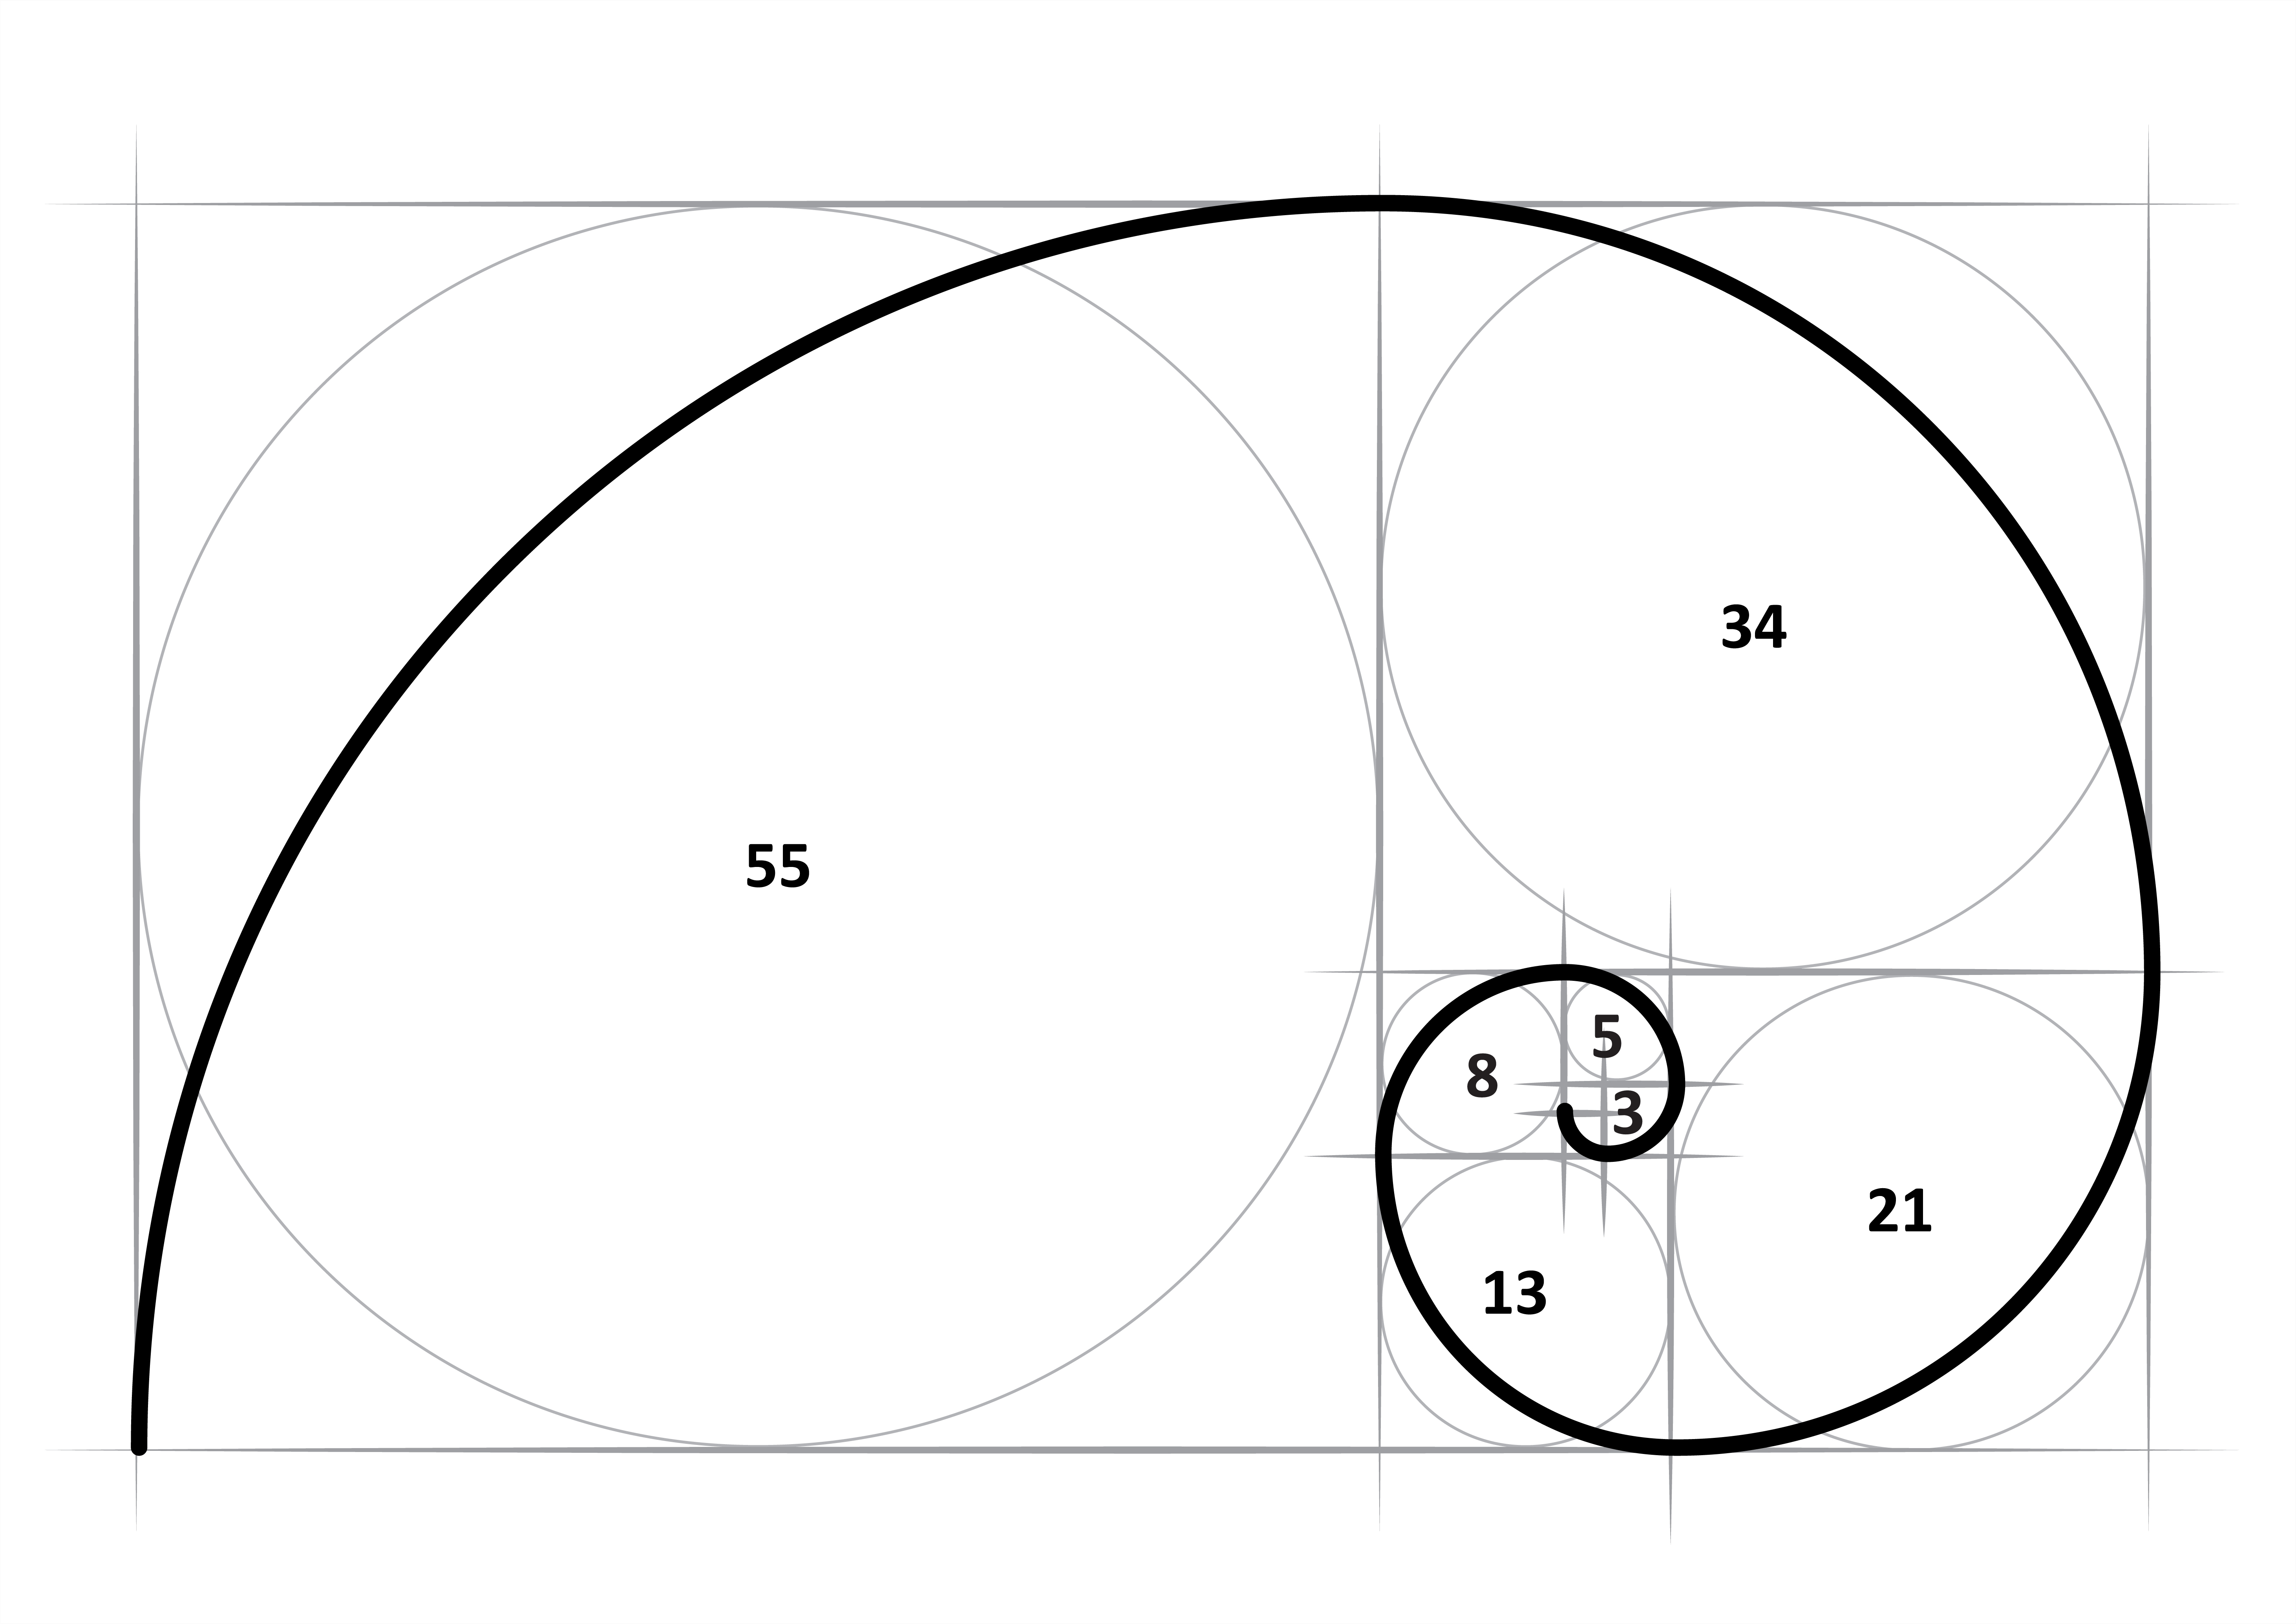
\includegraphics[scale=.17]{figuras/curvafibo.jpg}
\end{figure}

\inic Cada trecho da curva de Espiral tem comprimento seguindo os número da sequência de Fibonacci. A proporção Áurea é normalmente utilizada na arte, na arquitetura e no design por ser vista como agradável aos olhos humanos. Fica a cargo do Leitor mostrar que a solução da Recorrência de Fibonacci possui como coeficientes exatamente a proporção Àurea.

\inic Apresentaremos algumas curiosidades a repeito de aplicações naturais da sequência do número de ouro

\begin{enumerate}
    \item Cada novo pedaço da concha de uma caramujo tem formado possui a dimensão dos dois antecessores somados;
    \item Se um ser humano com altura mediana dividir sua altura pela distância entre o umbigo e a cabeça, o resultado será um número em torno de 1,618.
    \item As articulações de todos os dedos se relacionam na razão áurea, com exceção do polegar.
\end{enumerate}

\section{Casos especiais para Recorrência de segunda ordem}

\inic O primeiro caso que queremos abordar é quando $\varphi_1,\varphi_2 \notin \mathbb{R}$, neste caso teremos que fazer uma mudança para coordenadas polares que não será objetivo destas notas, mas para o leitor mais curioso consulte \cite{oliveira}. O Teorema \ref{iguais} mostra como determinar a solução da recorrência quando as raízes são iguais.

\begin{teo}
\label{iguais}
Se $\varphi_1 = \varphi_2 = \varphi$ são raízes de $\varphi^2-p\varphi-q = 0$ então $\varphi_n = c_1\varphi^n + c_2n\varphi^n$ é solução da recorrência associada a este polinômio.
\end{teo}

\begin{proof}
Seja $u_n$ ua solução de $x_n - px_{n-1} - qx_{n-2}$. Vamos tentar escrever $u_1$ e $u_2$ na forma
\begin{equation}
    u_n = c_1\varphi^n + c_2n\varphi^n
\end{equation}
então aplicando $u_1$ e $u_2$ na equação temos o sistema
\begin{equation}
    \begin{cases}
      c_1\varphi + c_2\varphi = u_1\\
      c_1\varphi^2 + 2c_2\varphi^2 = u_2
    \end{cases}
\end{equation}
\inic Solucionando o sistema temos $c_1 = \dfrac{2\varphi u_1 - u_2}{\varphi^2}$ e $c_2 = \dfrac{u_2 - \varphi u_1}{\varphi^2}$
que vale se $\varphi \neq 0$. Agora construímos a variável auxiliar $\nu_n$ que será a diferença entre a solução e $u_n$
\begin{equation}
    \nu_n = u_n - (c_1\varphi^n + c_2\varphi^n)
\end{equation}
queremos agora mostrar que $\nu_n = 0$. vamos resolver a equação
\begin{align*}
    \nu_n - p\nu_{n-1} - q \nu_{n-2} &= \underbrace{(u_n - pu_{n-1} - qu_{n-2})}_{=0} - c_1\varphi^{n-2}\underbrace{(\varphi^2 - p\varphi-q)}_{=0} - c_2n\varphi^{n-2}\underbrace{(\varphi^2 - p\varphi-q)}_{=0}\\
    - c_2\varphi^{n-2}\underbrace{(p\varphi - 2q)}_{=0}.
\end{align*}

\inic O último parentese é igual a zero pois $p=2\varphi$ e $q = -t^2$. Assim $\nu_1=\nu_2=0$ e $\nu_n - p\nu_{n-1} - q \nu_{n-2} = 0$ implica em $\nu_n= 0$. Logo
\begin{align*}
    \nu_n = 0\\
    u_n - (c_1\varphi^n + c_2n\varphi^n) = 0
    u_n = (c_1\varphi^n + c_2n\varphi^n)
\end{align*}
\end{proof}

\noindent \exercicio

\noindent [1] Qual o número máximo de regiões que $\mathnormal{n}$ retas que dividem o plano?

\noindent [2] Abaixo temos três figuras pentagonais: a primeira com 5 pontos a segunda com 12 pontos e a terceira com 22 pontos. Continuando esse processo de construção, a vigésima figura pentagonal terá 651 pontos. Quantos pontos terá a vigésima primeira figura?
\begin{figure}[H]
	\centering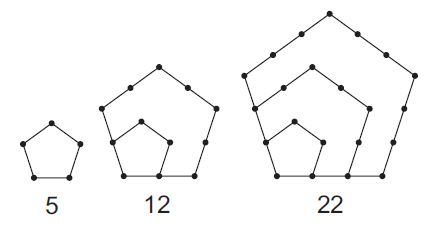
\includegraphics[scale=.8]{figuras/pent}
\end{figure}

\vspace{.5cm}

\noindent [3] Uma pessoa sai às compras e gasta na primeira loja que entra metade do que tem no bolso e mais um real. Na segunda loja gasta metade do que sobrou e mais um real. Na loja seguinte ocorre o mesmo. Entretanto, ao sair da terceira e última loja, a pessoa percebe que não tem dinheiro algum. Quantos reais ela possuía ao sair de casa?

\noindent [4] De quantas formas diferentes podemos organizar dominós em uma caixa $2\times \mathnormal{n}$?
\begin{figure}[H]
	\centering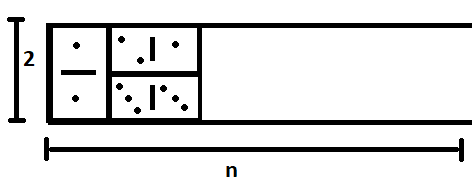
\includegraphics[scale=.65]{figuras/domino}
\end{figure}

\noindent [5] Uma função $f$ é definida para todos os inteiros positivos e satisfaz as condições: $f(1)=1996\,\, \text{e}\,\, \sum_{i=1}^{n}f(i) = n^2f(n)$ Calcule o valor exato de $f(1996)$.

\noindent [6] Sobre a sequência de Fibonacci, prove que:
\begin{enumerate}
    \item [(a)] A soma dos $n$ primeiros números de Fibonacci é igual a $F_{n+2} - 1$;
    \item [(b)] A soma dos $n$ primeiros números de Fibonacci com índices ímpares é igual a $F_{2n}$ e com índices pares é $F_{2n+1} -1$;
    \item [(c)] $F_{m+n} = F_{m-1}F_{n} + F_{n+1}F_{m}$ para todo $n \geq 1$ e $m>1$ (\textit{Sugestão}: use indução matemática em $n$)
\end{enumerate}

\noindent [7] Um coelho macho e uma fêmea nascem no início do ano. Assumindo que, depois de dois meses de idade, o casal de coelhos produz um par misto (um macho e uma fêmea), e então outro par misto de coelhos a cada mês, não ocorrem mortes durante o ano. Quantos coelhos teremos no fim do ano? (\textit{Sugestão:} Construa o casos mais simples primeiramente, para vocês procurar algum padrão dentro da sequência, logo após crie a fórmula de recorrência)



\chapter{Funções}

\inic Um dos conceitos mais importantes dentro do ambiente matemático é o conceito de funções que possui como ideia principal relacionar dois conjuntos, não necessariamente de números, mas conjunto de quaisquer objetos, desde que respeitem determinadas propriedades. A seguir temos a definição matemática deste objeto 

\section{Funções}

Antes de apresentarmos formalmente o conceito de função, considere a seguinte situação. Suponha que a altura de uma planta seja observada ao longo dos meses, produzindo os seguintes valores:

\begin{center}
    \begin{tabular}{c|c}
        \hline
        Mês & Altura \\
        \hline
        0 & $0{,}25$ m \\
        1 & $0{,}50$ m \\
        2 & $0{,}75$ m \\
        3 & $1{,}00$ m \\
        4 & $1{,}25$ m \\
        5 & $1{,}50$ m \\
        \hline
    \end{tabular}
\end{center}

Observe que, para cada mês considerado, existe uma única altura correspondente, isto é, não faz sentido a planta no mês 1 ter 0,5cm e 0,7cm de altura, por exemplo. Essa ideia de associar cada elemento de um conjunto a um único elemento de outro conjunto é a base do conceito de função.



\begin{defin}
    Considere dois conjuntos não vazios $A$ e $B$. Uma \textbf{função} de $A$ em $B$ é uma relação que associa a cada elemento $x\in A$ um único elemento $y\in B$. Denotamos uma função por $f:A\longrightarrow B$ onde $A$ é chamado de \textbf{domínio} da função e $B$ de \textbf{contradomínio}. Se o elemento $x\in A$ está associado ao elemento $y\in B$, escrevemos $y=f(x)$.
\end{defin}
Portanto, para que uma relação $f:A\to B$ seja uma função, cada elemento de $A$ deve estar associado a \textbf{um, e somente um}, elemento de $B$.

\begin{example}
    Alguns exemplos cotidianos ajudam a compreender quando uma relação é ou não uma função.

    \begin{enumerate}
        \item[(i)] Considere uma empresa que deseja preencher algumas vagas de emprego, sendo que cada vaga pode ser ocupada por apenas uma pessoa. Podemos considerar os conjuntos
        \[
            A=\{\text{vagas de emprego}\}
            \qquad\text{e}\qquad
            B=\{\text{funcionários da empresa}\}.
        \]
        Se associarmos cada vaga à pessoa que a ocupa, temos uma função $f:A\to B$, pois cada vaga está associada a uma única pessoa. Uma mesma pessoa pode, eventualmente, ocupar mais de uma função ou cargo, sem que isso viole a definição de função.

        \item[(ii)] Considere agora um conjunto de alunos de uma turma e suas respectivas datas de nascimento. Podemos definir
        \[
            A=\{\text{alunos da turma}\}
            \qquad\text{e}\qquad
            B=\{\text{datas do calendário}\}.
        \]
        A relação que associa cada aluno à sua data de nascimento é uma função $f:A\to B$, pois cada pessoa possui uma única data de nascimento. Observe que dois ou mais alunos podem ter nascido na mesma data, o que não viola a definição de função.

        \item[(iii)] Considere o conjunto de pessoas de uma cidade e o conjunto de seus números de telefone,
        \[
            A=\{\text{pessoas da cidade}\}
            \qquad\text{e}\qquad
            B=\{\text{números de telefone}\}.
        \]
        A relação que associa uma pessoa aos seus números de telefone, em geral, não é uma função, pois uma mesma pessoa pode possuir mais de um número de telefone. Assim, um mesmo elemento de $A$ poderia estar associado a mais de um elemento de $B$.

        \item[(iv)] Considere o conjunto de estudantes de uma universidade e o conjunto de disciplinas oferecidas,
        \[
            A=\{\text{estudantes}\}
            \qquad\text{e}\qquad
            B=\{\text{disciplinas}\}.
        \]
        A relação que associa cada estudante às disciplinas em que está matriculado não é, em geral, uma função, pois um estudante pode estar matriculado simultaneamente em várias disciplinas. Portanto, um mesmo elemento do domínio estaria associado a vários elementos do contradomínio.
    \end{enumerate}
\end{example}


\subsection{Representações de uma função}

Uma função pode ser representada de diferentes maneiras. As mais comuns são:

\begin{enumerate}
    \item[(i)] por meio de diagramas;
    \item[(ii)] por meio de uma expressão matemática;
    \item[(iii)] por meio de gráficos.
\end{enumerate}

Nos diagramas, cada elemento do conjunto $A$ deve possuir exatamente uma seta partindo dele. Elementos distintos de $A$, entretanto, podem estar associados ao mesmo elemento de $B$.

\begin{figure}[H]
    \centering
    \begin{tikzpicture}[
        every node/.style={font=\small},
        ponto/.style={circle, draw, minimum size=6mm, inner sep=0pt},
        >=stealth
    ]

        %--------------------------------
        % (a) É função
        %--------------------------------
        \node at (1.5,1) {\textbf{É função}};
        \node at (0,0.7) {$A$};
        \node at (3,0.7) {$B$};

        \foreach \y/\v in {0/1,-1/2,-2/3,-3/4,-4/5}
            \node[ponto] (a\v) at (0,\y) {\v};

        \foreach \y/\v in {0/1,-1/2,-2/3,-3/4,-4/5}
            \node[ponto] (b\v) at (3,\y) {\v};

        \draw[->] (a1) -- (b2);
        \draw[->] (a2) -- (b3);
        \draw[->] (a3) -- (b4);
        \draw[->] (a4) -- (b5);
        \draw[->] (a5) -- (b1);


        %--------------------------------
        % (b) É função
        %--------------------------------
        \begin{scope}[xshift=6cm]

            \node at (1.5,1) {\textbf{É função}};
            \node at (0,0.7) {$A$};
            \node at (3,0.7) {$B$};

            \foreach \y/\v in {0/1,-1/2,-2/3,-3/4,-4/5}
                \node[ponto] (c\v) at (0,\y) {\v};

            \foreach \y/\v in {0/1,-1/2,-2/3,-3/4,-4/5}
                \node[ponto] (d\v) at (3,\y) {\v};

            \draw[->] (c1) -- (d2);
            \draw[->] (c2) -- (d2);
            \draw[->] (c3) -- (d4);
            \draw[->] (c4) -- (d4);
            \draw[->] (c5) -- (d4);

        \end{scope}


        %--------------------------------
        % (c) Não é função
        %--------------------------------
        \begin{scope}[xshift=12cm]

            \node at (1.5,1) {\textbf{Não é função}};
            \node at (0,0.7) {$A$};
            \node at (3,0.7) {$B$};

            \foreach \y/\v in {0/1,-1/2,-2/3,-3/4,-4/5}
                \node[ponto] (e\v) at (0,\y) {\v};

            \foreach \y/\v in {0/1,-1/2,-2/3,-3/4,-4/5}
                \node[ponto] (f\v) at (3,\y) {\v};

            \draw[->] (e1) -- (f1);
            \draw[->] (e2) -- (f2);
            \draw[->] (e2) -- (f4);
            \draw[->] (e3) -- (f3);
            \draw[->] (e4) -- (f4);
            \draw[->] (e5) -- (f5);

        \end{scope}

    \end{tikzpicture}
    \caption{Exemplos de relações entre os conjuntos $A$ e $B$. Nos dois primeiros casos, cada elemento de $A$ está associado a um único elemento de $B$, caracterizando uma função. No último caso, o elemento $2\in A$ está associado a dois elementos distintos de $B$ e, portanto, a relação não é uma função.}
    \label{fig:diagramas-funcao}
\end{figure}

\subsection{Domínio de uma função}

Considere uma função $f:A\longrightarrow B$. Chamamos de \textbf{domínio} de $f$, denotado por $D(f)$, o conjunto formado por todos os valores de $x$ para os quais a função está definida. Quando uma função é apresentada apenas por meio de sua expressão algébrica, devemos determinar quais valores de $x$ tornam essa expressão bem definida.

\begin{figure}[H]
    \centering
    \begin{tikzpicture}[
        >=stealth,
        ponto/.style={circle, draw, minimum size=7mm, inner sep=0pt},
        selecionado/.style={circle, draw, fill=red!35, minimum size=7mm, inner sep=0pt},
        every node/.style={font=\small}
    ]

        % ==================================================
        % DOMÍNIO
        % ==================================================

        \node[font=\bfseries] at (1.5,2) {Domínio};

        \node at (0,1.3) {$A$};
        \node at (3,1.3) {$B$};

        % Elementos de A
        \node[selecionado] (a1) at (0,0.5) {$1$};
        \node[selecionado] (a2) at (0,-0.5) {$2$};
        \node[selecionado] (a3) at (0,-1.5) {$3$};
        \node[ponto]       (a4) at (0,-2.5) {$4$};
        \node[ponto]       (a5) at (0,-3.5) {$5$};

        % Elementos de B
        \node[ponto] (b1) at (3,0.5) {$1$};
        \node[ponto] (b2) at (3,-0.5) {$2$};
        \node[ponto] (b3) at (3,-1.5) {$3$};
        \node[ponto] (b4) at (3,-2.5) {$4$};
        \node[ponto] (b5) at (3,-3.5) {$5$};

        % Setas
        \draw[->] (a1) -- (b1);
        \draw[->] (a2) -- (b2);
        \draw[->] (a3) -- (b3);
    \end{tikzpicture}

    \caption{Representação do domínio e da imagem de uma relação. As bolinhas destacadas em vermelho representam os elementos que pertencem ao domínio, as que não estão em vermelho são pertencem ao conjunto A, porém não ao domínio.}
\end{figure}

Em particular, devemos observar algumas restrições importantes, que em geral são as que aparecem em problemas.

\begin{enumerate}
    \item[(i)] Denominadores não podem ser iguais a zero;
    \item[(ii)] Raízes de índice par não podem possuir radicando negativo, quando trabalhamos no conjunto dos números reais.
\end{enumerate}

\begin{example}
    Considere a função
    \begin{equation}
        f(x)=\frac{1}{x-1}.
    \end{equation}
    Para que a função esteja definida, devemos ter
    \begin{align*}
        x-1 &\neq 0 \\
        x &\neq 1.
    \end{align*}
    Portanto,
    \begin{equation}
        D(f)=\{x\in\mathbb{R}:x\neq1\}
        =\mathbb{R}\setminus\{1\}.
    \end{equation}

    Por exemplo,
    \begin{align*}
        f(2)&=\frac{1}{2-1}=1,
        &
        f(3)&=\frac{1}{3-1}=\frac{1}{2}.
    \end{align*}
\end{example}

\begin{example}
    Considere a função
    \begin{equation}
        f(x)=\sqrt{2x-4}.
    \end{equation}
    Como estamos trabalhando em $\mathbb{R}$, devemos ter
    \begin{align*}
        2x-4 &\geq 0 \\
        2x &\geq 4 \\
        x &\geq 2.
    \end{align*}
    Portanto,
    \begin{equation*}
        D(f)=\{x\in\mathbb{R}:x\geq2\}=[2,\infty).
    \end{equation*}
\end{example}

\subsection{Conjunto Imagem}

Considere novamente uma função $f:A\to B$. Chamamos de \textbf{imagem} de $f$, denotada por $\operatorname{Im}(f)$, o conjunto formado pelos elementos de $B$ que estão associados a pelo menos um elemento do domínio.

Formalmente,
\begin{equation}
    \operatorname{Im}(f)
    =\{y\in B:\text{ existe }x\in A\text{ tal que }y=f(x)\}.
\end{equation}

Observe que a imagem de uma função é sempre um subconjunto de seu contradomínio, isto é,
\begin{equation}
    \operatorname{Im}(f)\subseteq B.
\end{equation}

\begin{figure}[H]
    \centering
    \begin{tikzpicture}[
        >=stealth,
        ponto/.style={circle, draw, minimum size=7mm, inner sep=0pt},
        selecionado/.style={circle, draw, fill=red!35, minimum size=7mm, inner sep=0pt},
        every node/.style={font=\small}
    ]

       


        % ==================================================
        % IMAGEM
        % ==================================================

        \begin{scope}[xshift=7cm]

            \node[font=\bfseries] at (1.5,2) {Imagem};

            \node at (0,1.3) {$A$};
            \node at (3,1.3) {$B$};

            % Elementos de A
            \node[ponto] (c1) at (0,0.5) {$1$};
            \node[ponto] (c2) at (0,-0.5) {$2$};
            \node[ponto] (c3) at (0,-1.5) {$3$};
            \node[ponto] (c4) at (0,-2.5) {$4$};
            \node[ponto] (c5) at (0,-3.5) {$5$};

            % Elementos de B
            \node[selecionado] (d1) at (3,0.5) {$1$};
            \node[selecionado] (d2) at (3,-0.5) {$2$};
            \node[selecionado] (d3) at (3,-1.5) {$3$};
            \node[ponto]       (d4) at (3,-2.5) {$4$};
            \node[ponto]       (d5) at (3,-3.5) {$5$};

            % Setas
            \draw[->] (c1) -- (d1);
            \draw[->] (c2) -- (d2);
            \draw[->] (c3) -- (d3);

        \end{scope}

    \end{tikzpicture}

    \caption{Representação do domínio e da imagem de uma relação. As bolinhas destacadas em vermelho representam os elementos que pertencem ao domínio, à esquerda, e à imagem, à direita.}
\end{figure}


\begin{example}
    Considere a função
    \begin{equation}
        f:\mathbb{R}\longrightarrow\mathbb{R},
        \qquad
        f(x)=x^2-1.
    \end{equation}
    Como $x^2\geq0$ para todo $x\in\mathbb{R}$, temos
    \begin{equation}
        x^2-1\geq-1.
    \end{equation}
    Além disso, todo valor real maior ou igual a $-1$ pode ser obtido pela função. Portanto,
    \begin{equation}
        \operatorname{Im}(f)
        =\{y\in\mathbb{R}:y\geq-1\}
        =[-1,\infty).
    \end{equation}
\end{example}

Uma função é caracterizada por três elementos fundamentais
\begin{enumerate}
    \item seu \textbf{domínio};
    \item seu \textbf{contradomínio};
    \item sua \textbf{lei de formação}, isto é, a regra que determina $f(x)$ para cada $x$ pertencente ao domínio.
\end{enumerate}

Assim, ao escrevermos
\begin{equation}
    f:A\longrightarrow B,
    \qquad
    x\longmapsto f(x),
\end{equation}
estamos especificando o domínio $A$, o contradomínio $B$ e a regra que associa cada $x\in A$ ao seu respectivo valor $f(x)\in B$.

\subsection{Gráfico}

Considere uma função $f:A\to B$. Chamamos de \textbf{gráfico de $f$} o conjunto de todos os pares ordenados $(x,f(x))$, com $x\in A$. Isto é,
\begin{equation*}
    G(f)=\{(x,f(x)):x\in A\}.
\end{equation*}

Geometricamente, quando $A$ e $B$ são subconjuntos de $\mathbb{R}$, cada par $(x,f(x))$ pode ser representado como um ponto no plano cartesiano. O conjunto de todos esses pontos constitui a representação gráfica da função.

Observe que, para cada valor $x$ pertencente ao domínio, existe um único valor $f(x)$ associado. Consequentemente, uma reta vertical não pode intersectar o gráfico de uma função em mais de um ponto. Essa observação é conhecida como \textbf{teste da reta vertical}.

\begin{figure}[H]
    \centering
    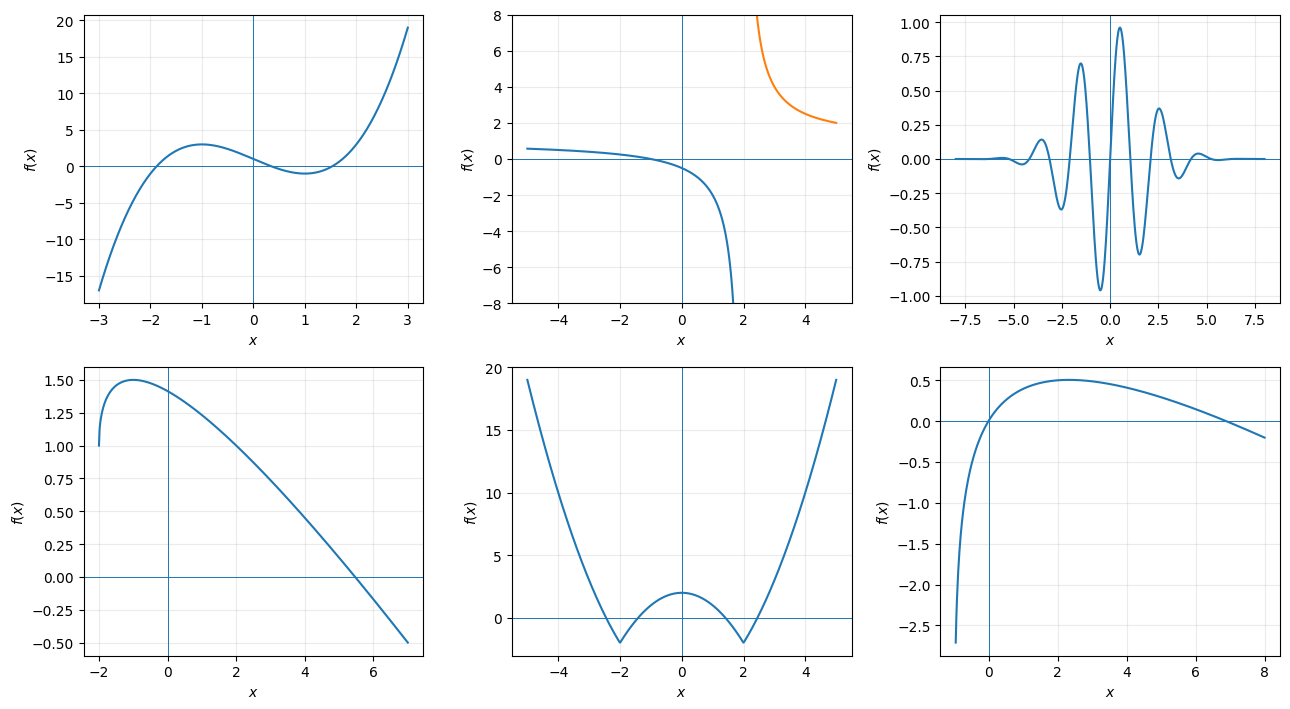
\includegraphics[width=\textwidth]{figuras/graficos_funcoes_3x2.png}
    \caption{Exemplos de representações gráficas de diferentes funções reais. Cada ponto do gráfico possui a forma $(x,f(x))$, em que $x$ pertence ao domínio da respectiva função.}
    \label{fig:exemplos-graficos-funcoes}
\end{figure}

\section{Função afim}

Até o momento, estudamos funções de maneira geral, apresentando conceitos como domínio, contradomínio, imagem e representação gráfica. A partir de agora, começaremos a afunilar nosso estudo, considerando algumas classes particulares de funções que aparecem com frequência tanto na Matemática quanto na modelagem de fenômenos reais.

Uma das classes mais simples e importantes é a das \textbf{funções afins}. Diversos fenômenos podem ser modelados, ao menos aproximadamente, por meio de uma função afim. Além de sua simplicidade matemática, um dos principais motivos para o interesse nesse tipo de modelo é sua fácil interpretabilidade, uma vez que seus parâmetros possuem significados claros e permitem compreender diretamente como uma variável se modifica em função de outra.



\begin{defin}
    Chamamos de \textbf{função afim} toda função $f:\mathbb{R}\to\mathbb{R}$ que pode ser escrita na forma
\begin{equation*}
    f(x)=ax+b,
\end{equation*}
em que $a,b\in\mathbb{R}$ são constantes.
\end{defin}

\begin{figure}[H]
    \centering
    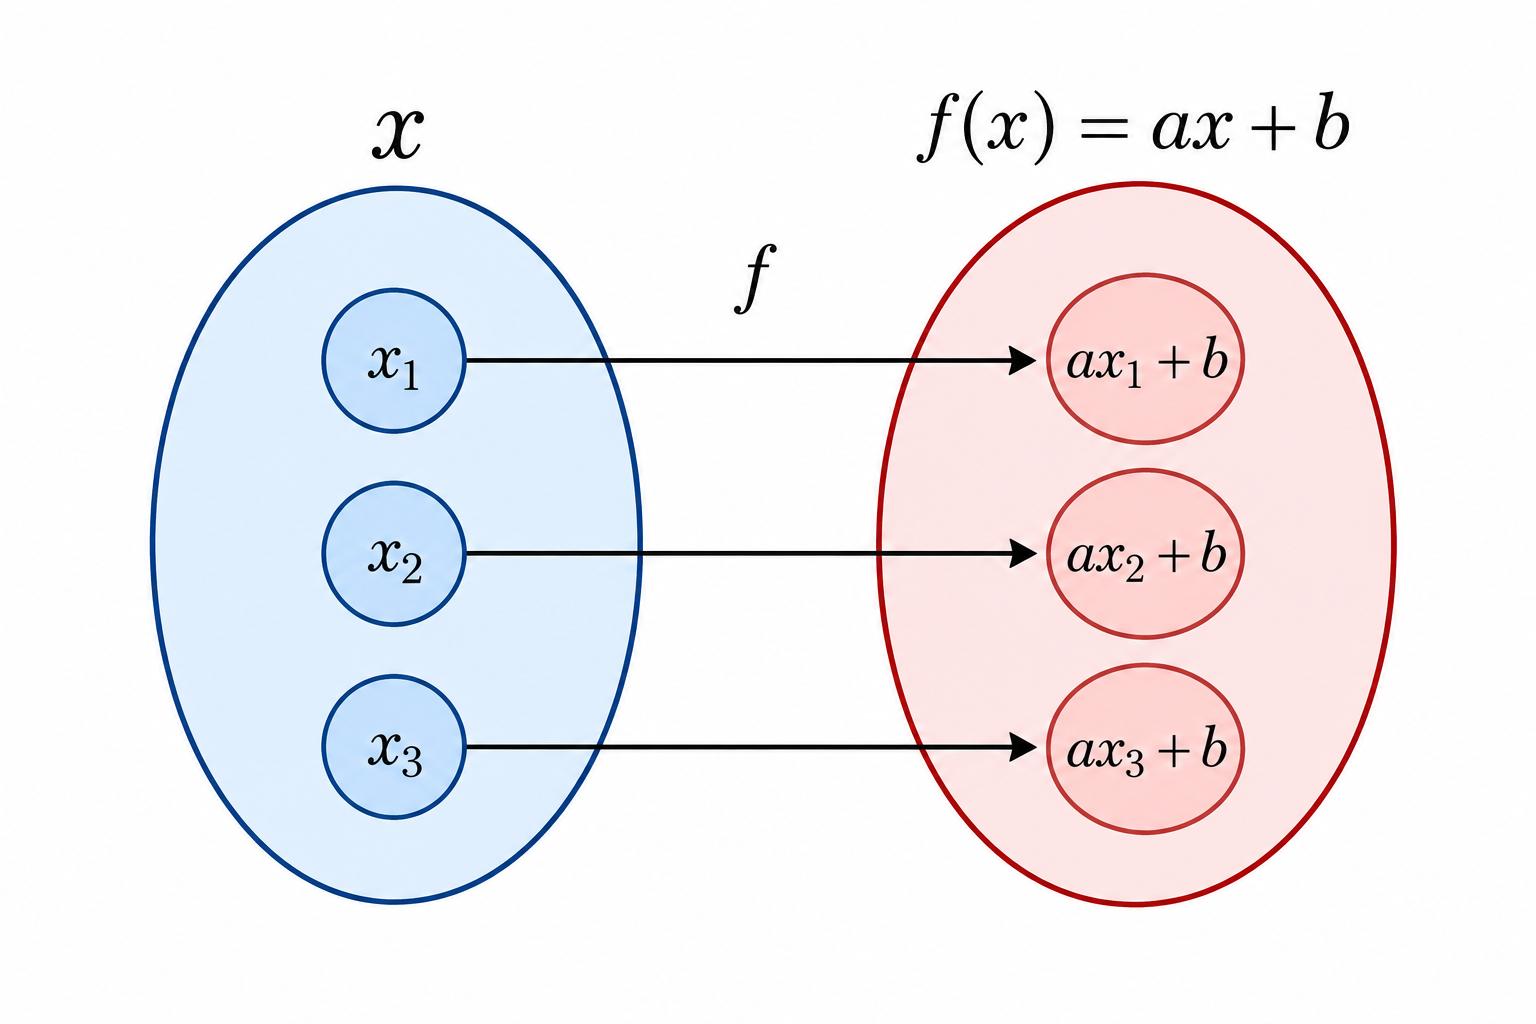
\includegraphics[width=0.8\textwidth]{figuras/diagrama_afim.png}
    \caption{Representação da função afim $f(x)=ax+b$ por meio de um diagrama.}
    \label{fig:diagrama_afim}
\end{figure}

O parâmetro $a$ é chamado de \textbf{coeficiente angular} e determina a taxa de variação da função. Em outras palavras, ele indica quanto o valor de $f(x)$ varia quando aumentamos $x$ em uma unidade. De fato,
\begin{equation*}
    f(x+1)-f(x)=a.
\end{equation*}
Assim, quando $a>0$, a função cresce à medida que $x$ aumenta; quando $a<0$, a função decresce; e, quando $a=0$, temos uma função constante.

O parâmetro $b$ é chamado de \textbf{coeficiente linear} e representa o valor assumido pela função quando $x=0$. De fato,
\begin{equation*}
    f(0)=a\cdot0+b=b.
\end{equation*}

Dessa forma, os dois parâmetros possuem interpretações bastante naturais: enquanto $a$ descreve a \textbf{taxa de variação} da função, $b$ determina seu \textbf{valor inicial}, isto é, o valor da função quando $x=0$.

\begin{example}
    Considere a função afim
    \begin{equation*}
        f(x)=2x+3.
    \end{equation*}
    Podemos estar interessados tanto em determinar a imagem de um determinado valor de $x$ quanto em realizar o processo inverso, isto é, determinar qual valor de $x$ possui uma imagem previamente especificada.

    Por exemplo, para determinar a imagem de $x=1$, basta substituir esse valor na função:
    \begin{align*}
        f(1)&=2\cdot1+3=5.
    \end{align*}
    Portanto, a imagem de $1$ pela função $f$ é $5$.

    Agora, suponha que desejamos determinar qual valor de $x$ possui imagem igual a $10$. Nesse caso, procuramos $x$ tal que $f(x)=10$. Assim,
    \begin{align*}
        2x+3&=10 \\
        2x&=7 \\
        x&=\frac{7}{2}.
    \end{align*}
    Portanto,
    \begin{equation*}
        f\left(\frac{7}{2}\right)=10.
    \end{equation*}

    Dessa forma, quando conhecemos $x$, podemos calcular diretamente sua imagem $f(x)$. Por outro lado, quando conhecemos o valor da imagem, podemos determinar o valor de $x$ correspondente resolvendo a equação $f(x)=y$.
\end{example}


Geometricamente, portanto, $b$ determina o ponto em que o gráfico da função intersecta o eixo vertical. Agora provaremos no Teorema~\ref{reta}  que o gráfico da função afim é dado por uma reta. 

\begin{teo}
\label{reta}
    Seja $f:\mathbb{R}\to\mathbb{R}$ uma função afim dada por $f(x)=ax+b$, com $a,b\in\mathbb{R}$. Então o gráfico de $f$ é uma reta no plano cartesiano.
\end{teo}

\begin{proof}
    Considere dois pontos distintos do gráfico de $f$,
    \begin{equation*}
        P_1=(x_1,f(x_1))
        \qquad\text{e}\qquad
        P_2=(x_2,f(x_2)),
    \end{equation*}
    com $x_1\neq x_2$. O coeficiente angular da reta que passa por esses dois pontos é dado por
    \begin{align*}
        \frac{f(x_2)-f(x_1)}{x_2-x_1}
        &=\frac{(ax_2+b)-(ax_1+b)}{x_2-x_1}
        =\frac{a(x_2-x_1)}{x_2-x_1}
        =a.
    \end{align*}
    Portanto, quaisquer dois pontos distintos do gráfico determinam sempre o mesmo coeficiente angular $a$. Além disso, como
    \begin{equation*}
        f(0)=b,
    \end{equation*}
    o gráfico passa pelo ponto $(0,b)$. Consequentemente, todos os pontos $(x,f(x))$ satisfazem a equação
    \begin{equation*}
        y=ax+b,
    \end{equation*}
    que é a equação de uma reta de coeficiente angular $a$ e que intersecta o eixo vertical no ponto $(0,b)$. Logo, o gráfico de $f$ é uma reta.
\end{proof}
A Figura~\ref{fig:grade_funcoes_afins} mostra vários comportamentos da reta da função $f(x) = ax+b$ 

\begin{figure}[H]
    \centering
    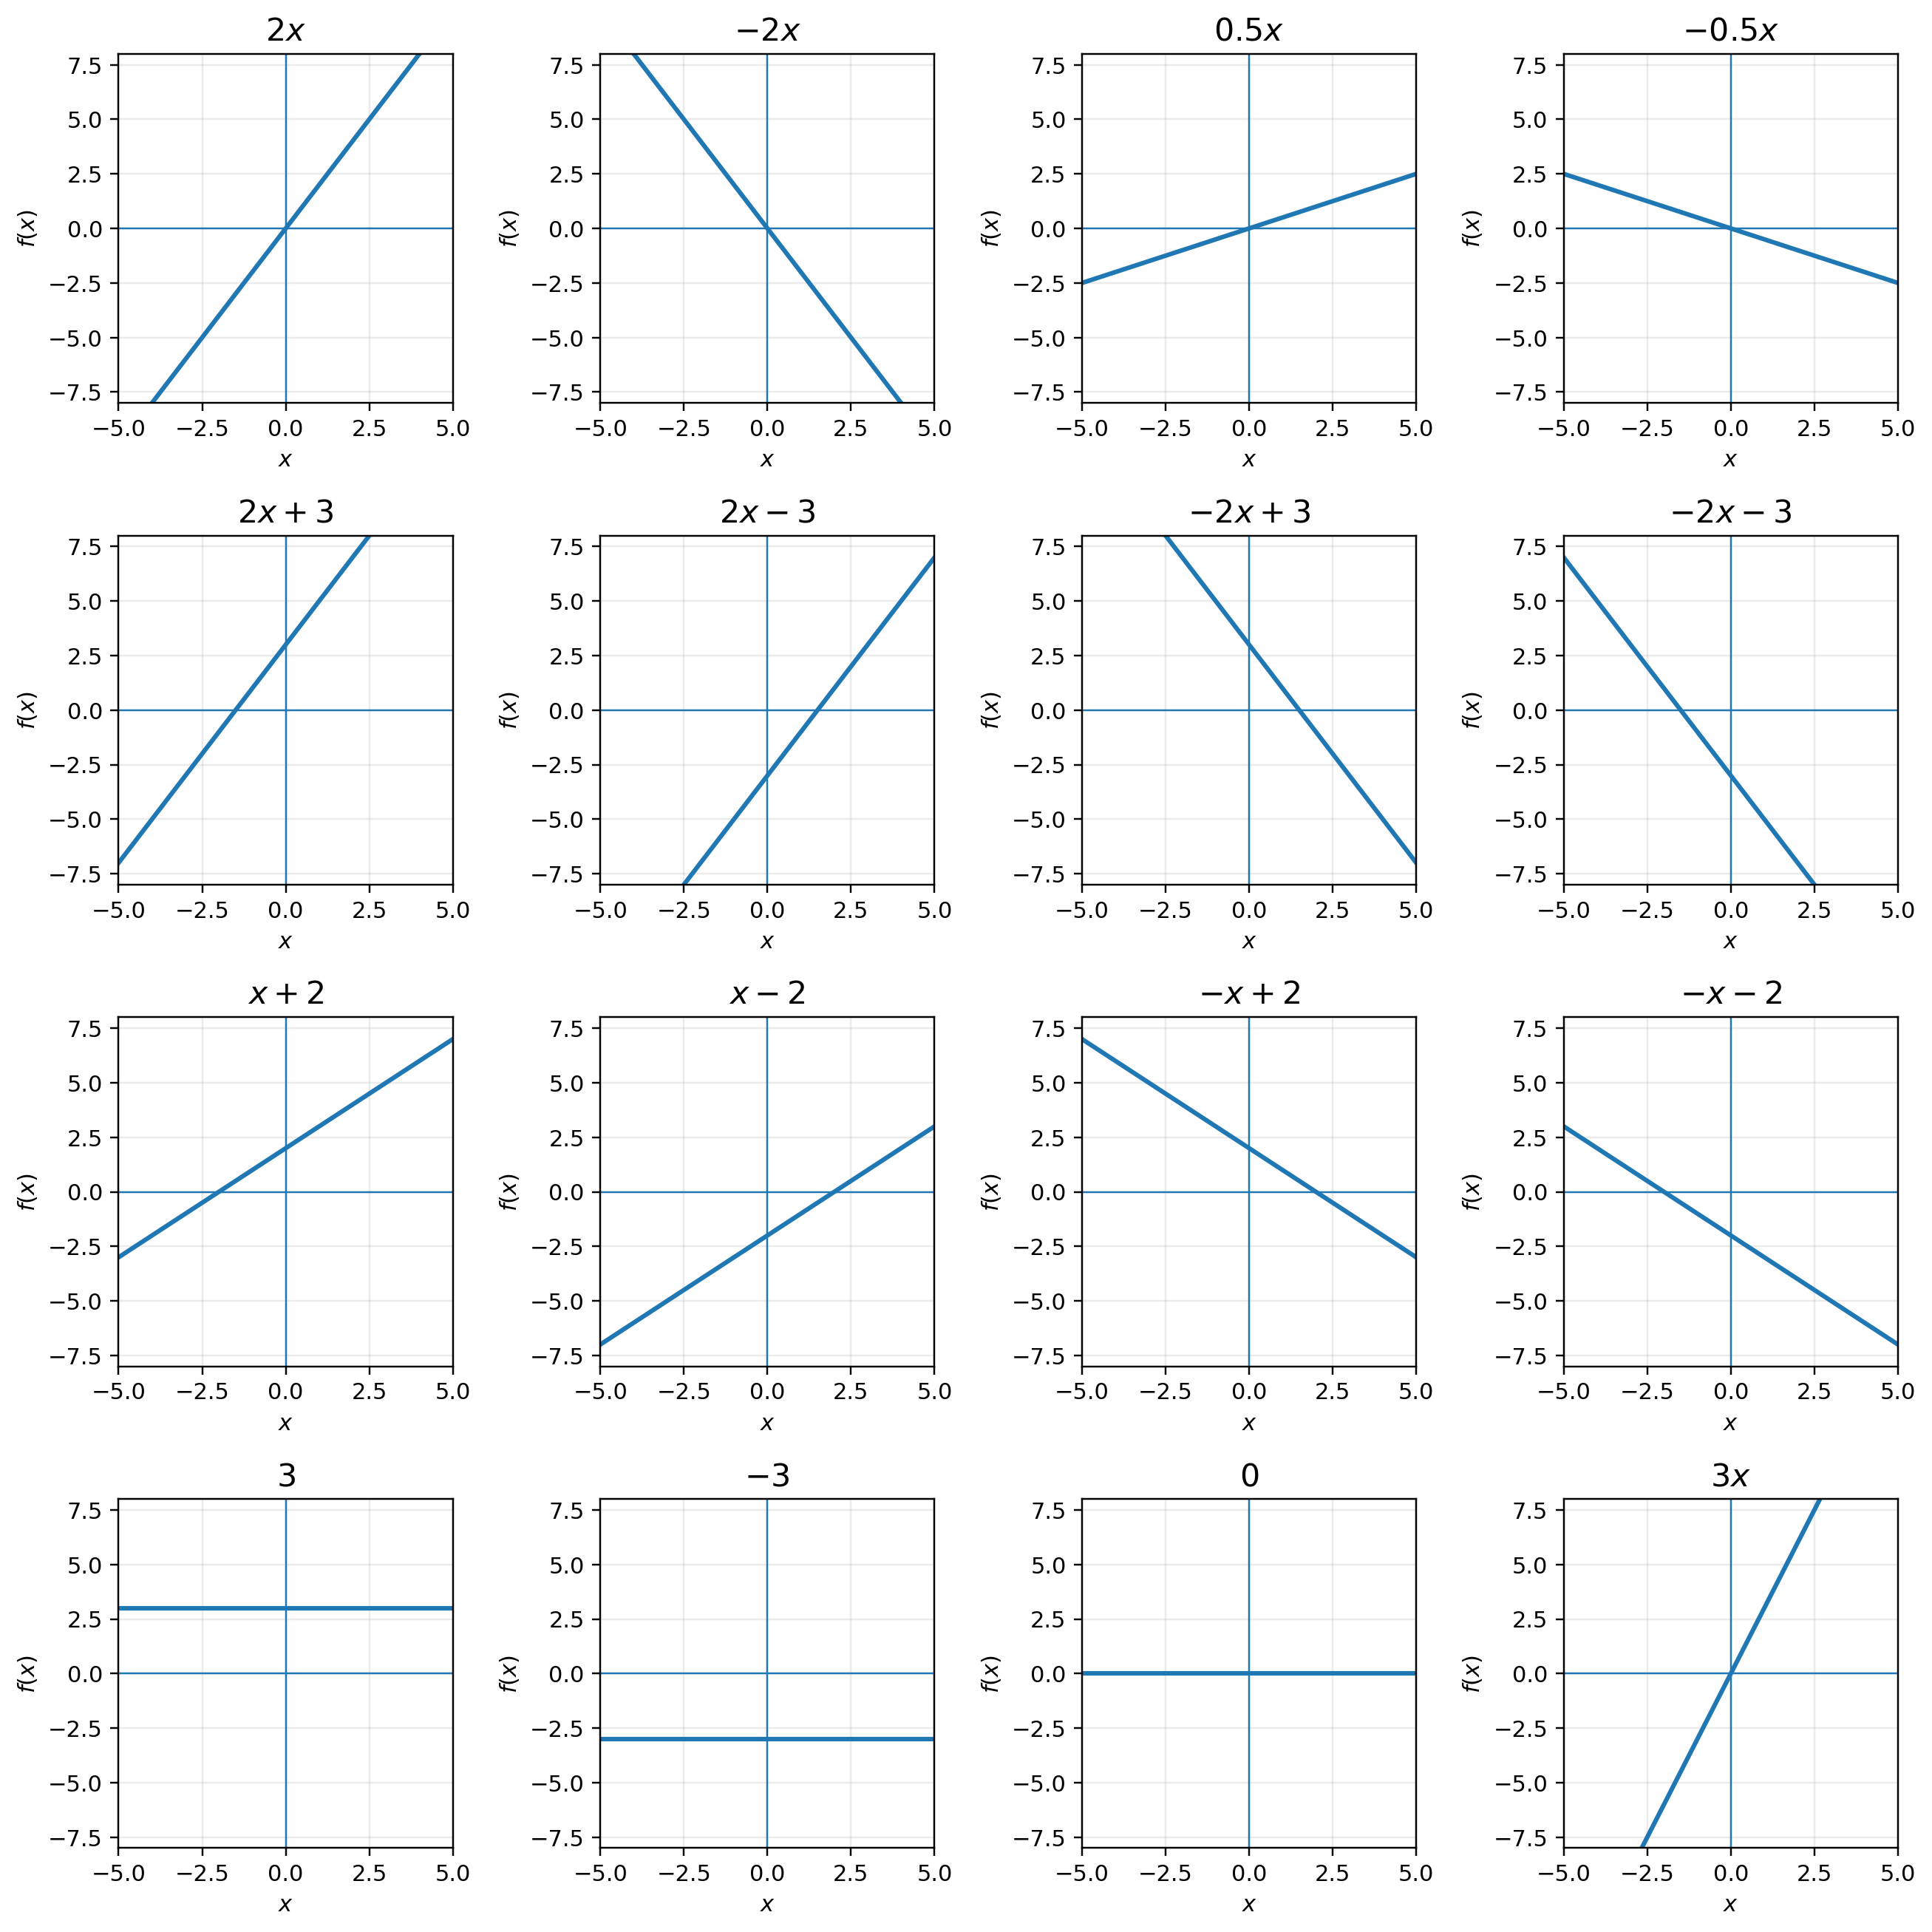
\includegraphics[width=0.79\textwidth]{figuras/grade_funcoes_afins_4x4.png}
    \caption{Exemplos de gráficos de funções afins para diferentes valores dos coeficientes $a$ e $b$.}
    \label{fig:grade_funcoes_afins}
\end{figure}

\subsection{Aplicações da função afim}

A função afim pode ser utilizada para representar situações nas quais uma quantidade varia a uma taxa constante em relação a outra. Nesses casos, o coeficiente angular $a$ representa justamente essa taxa de variação, enquanto o coeficiente linear $b$ representa o valor inicial da quantidade estudada. Vejamos alguns exemplos.

\begin{example}
    Considere uma obra na qual a utilização de concreto envolve um custo fixo de R\$ $1.200,00$, referente à mobilização dos equipamentos, além de um custo de R\$ $450,00$ para cada metro cúbico de concreto utilizado.

    Se $x$ representa o volume de concreto utilizado, em metros cúbicos, e $C(x)$ representa o custo total, podemos organizar alguns valores na seguinte tabela:

    \begin{center}
        \begin{tabular}{c|c}
            \hline
            Volume ($\text{m}^3$) & Custo (R\$) \\
            \hline
            0  & $1.200$ \\
            2  & $2.100$ \\
            4  & $3.000$ \\
            6  & $3.900$ \\
            8  & $4.800$ \\
            10 & $5.700$ \\
            \hline
        \end{tabular}
    \end{center}

    Observe que, a cada aumento de $1\,\text{m}^3$ no volume de concreto, o custo aumenta R\$ $450,00$. Além disso, quando $x=0$, ainda existe o custo fixo de R\$ $1.200,00$. Dessa forma, o modelo algébrico é dado por
    \begin{equation*}
        C(x)=450x+1200.
    \end{equation*}

    Nesse modelo, $a=450$ representa o custo adicional por metro cúbico de concreto, enquanto $b=1200$ representa o custo inicial da operação.

    \begin{figure}[H]
        \centering
        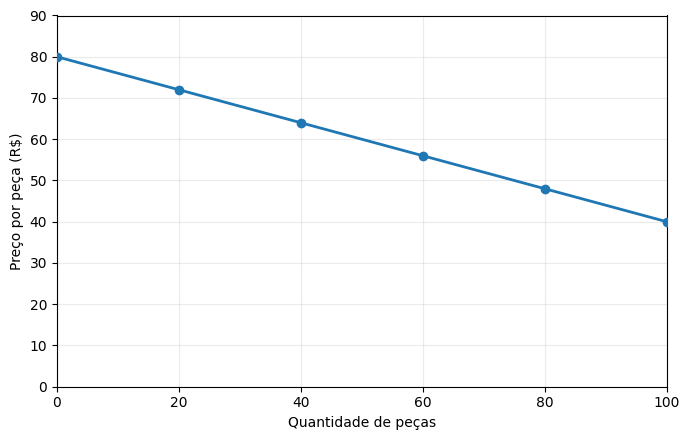
\includegraphics[width=0.7\textwidth]{figuras/exemplo_afim_civil.png}
        \caption{Custo em função do volume de concreto utilizado.}
        \label{fig:afim_engenharia}
    \end{figure}
\end{example}

\begin{example}
    Considere um modelo simplificado para representar a energia disponível de um jogador durante uma partida de futebol. Suponha que o jogador inicie a partida com $100\%$ de energia disponível e que, segundo o modelo, esse percentual diminua $0{,}6$ ponto percentual a cada minuto de jogo.

    Se $t$ representa o tempo de jogo, em minutos, e $E(t)$ representa o percentual de energia disponível, temos:

    \begin{center}
        \begin{tabular}{c|c}
            \hline
            Tempo (min) & Energia disponível (\%) \\
            \hline
            0  & $100$ \\
            15 & $91$ \\
            30 & $82$ \\
            45 & $73$ \\
            60 & $64$ \\
            75 & $55$ \\
            90 & $46$ \\
            \hline
        \end{tabular}
    \end{center}

    Como a energia diminui $0{,}6$ ponto percentual por minuto, temos $a=-0{,}6$. Além disso, no instante inicial, $E(0)=100$. Portanto, o modelo é
    \begin{equation*}
        E(t)=-0{,}6t+100.
    \end{equation*}

    Nesse exemplo, o coeficiente negativo indica que a variável estudada diminui com o passar do tempo. O coeficiente $b=100$, por sua vez, representa a energia disponível no início da partida.

    \begin{figure}[H]
        \centering
        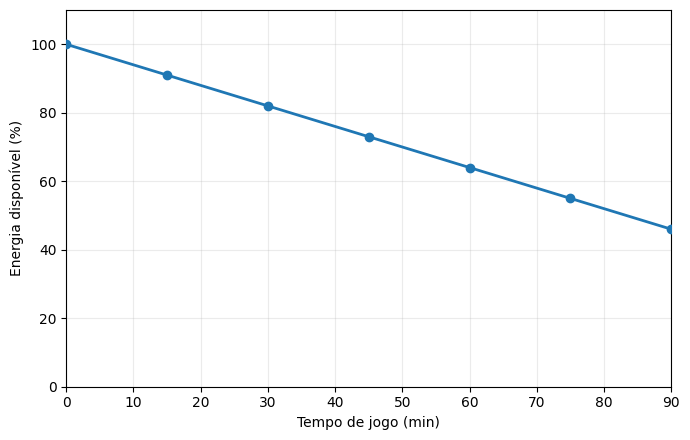
\includegraphics[width=0.7\textwidth]{figuras/exemplo_afim_futebol.png}
        \caption{Modelo simplificado da energia disponível de um jogador em função do tempo de jogo.}
        \label{fig:afim_futebol}
    \end{figure}
\end{example}

\begin{example}
    Considere uma confecção que estabelece o preço por peça de determinado produto de acordo com a quantidade encomendada. Suponha que o preço inicial seja de R\$ $80,00$ por peça e que, em uma determinada faixa de produção, a empresa conceda um desconto de R\$ $0,40$ no preço unitário para cada unidade acrescentada ao pedido.

    Se $q$ representa a quantidade de peças e $P(q)$ representa o preço unitário, alguns valores desse modelo são:

    \begin{center}
        \begin{tabular}{c|c}
            \hline
            Quantidade de peças & Preço por peça (R\$) \\
            \hline
            0   & $80$ \\
            20  & $72$ \\
            40  & $64$ \\
            60  & $56$ \\
            80  & $48$ \\
            100 & $40$ \\
            \hline
        \end{tabular}
    \end{center}

    Nesse caso, cada unidade adicional reduz o preço unitário em R\$ $0,40$. Logo, a taxa de variação é $a=-0{,}4$. Como o valor inicial utilizado pelo modelo é $b=80$, obtemos
    \begin{equation*}
        P(q)=-0{,}4q+80.
    \end{equation*}

    Novamente, o sinal negativo do coeficiente angular indica uma relação decrescente: quanto maior a quantidade encomendada, menor é o preço por peça, dentro da faixa em que o modelo é considerado válido.

    \begin{figure}[H]
        \centering
        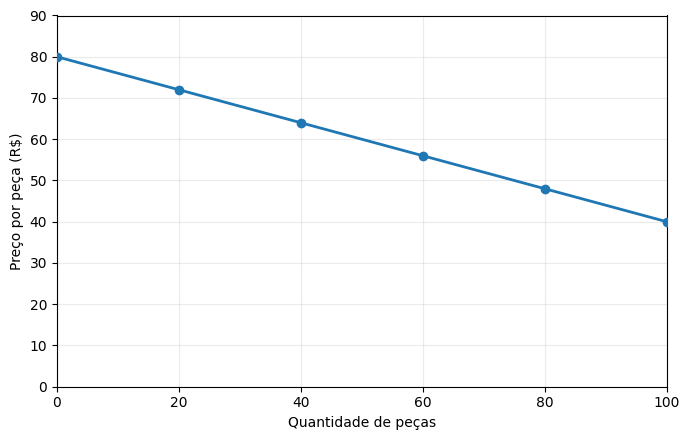
\includegraphics[width=0.7\textwidth]{figuras/exemplo_afim_moda.png}
        \caption{Preço unitário em função da quantidade de peças encomendadas.}
        \label{fig:afim_moda}
    \end{figure}
\end{example}




\bibliographystyle{ieeetr} % plain abbrv newapa apa apalike plainnat amsplain abbrvnat unsrtnat ieeetr
\bibliography{bibliografia}
%\printbibliography 

\end{document}
